
\chapter{Lifelong Word Representation Learning}
\label{chap3:word}

Learning word embeddings \cite{mnih2007three,mikolov2013efficient,mikolov2013distributed,pennington2014glove}
has received a great deal of attention due to its success in numerous NLP applications, e.g., named entity recognition \cite{sienvcnik2015adapting}, sentiment analysis \cite{maas2011learning} and syntactic parsing \cite{durrett2015neural}.
The key to the success of word embeddings is that a large-scale corpus can be turned into a huge number (e.g., billions) of training examples.

There are two implicit assumptions are often made about the effectiveness of embeddings to down-stream tasks: 
1) the training corpus for embedding is available and much larger than the training data of the down-stream task; 2) the topic (domain) of the embedding corpus is closely aligned with the topic of the downstream task.
However, many real-life applications do not meet both assumptions.

In most cases, the in-domain corpus is of limited size, which is insufficient for training good embeddings. 
In applications, researchers and practitioners often simply use some general-purpose embeddings trained using a very large general-purpose corpus (which satisfies the first assumption) covering almost all possible topics, e.g., the GloVe embeddings \cite{pennington2014glove} trained using 840 billion tokens covering almost all topics/domains on the Web. Such embeddings have been shown to work reasonably well in many domain-specific tasks. This is not surprising as the meanings of a word are largely shared across domains and tasks. However, this solution violates the second assumption, which often leads to sub-optimal results for domain-specific tasks, as shown in our experiments.
One obvious explanation for this is that the general-purpose embeddings do provide some useful information for many words in the domain task, but their embedding representations may not be ideal for the domain and in some cases, they may even conflict with the meanings of the words in the task domain because words often have multiple senses or meanings.
For example, we have a task in the programming domain, which has the word ``Java''. A large-scale general-purpose corpus, which is very likely to include texts about coffee shops, supermarkets, the Java island of Indonesia, etc., can easily squeeze the room for representing ``Java''' context words like ``function'', ``variable'' or ``Python'' in the programming domain.
This results in a poor representation of the word ``Java'' for the programming task.  

\section{Motivation}
\label{chap3:sec:intro}

Thus, learning high-quality domain word embeddings is important for achieving good performance in many NLP tasks. General-purpose embeddings trained on large-scale corpora are often sub-optimal for domain-specific applications. However, domain-specific tasks often do not have large in-domain corpora for training high-quality domain embeddings.

As such, we propose a novel \textit{lifelong learning} setting for domain embedding. That is, when performing the new domain embedding, the system has seen many past domains, and it tries to expand the new in-domain corpus by exploiting the corpora from the past domains via meta-learning. The proposed meta-learner characterizes the similarities of the contexts of the same word in many domain corpora, which helps retrieve relevant data from the past domains to expand the new domain corpus. 

To solve this problem and also the limited in-domain corpus size problem, cross-domain embeddings have been investigated \cite{bollegala-maehara-kawarabayashi:2015:ACL-IJCNLP,yang-lu-zheng:2017:EMNLP2017,bollegala2017think} via transfer learning \cite{pan2010survey}.
These methods allow some in-domain words to leverage the general-purpose embeddings in the hope that the meanings of these words in the general-purpose embeddings do not deviate much from the in-domain meanings of these words. The embeddings of these words can thus be improved. However, these methods cannot improve the embeddings of many other words with domain-specific meanings (e.g., ``Java'').
Further, some words in the general-purpose embeddings may carry meanings that are different from those in the task domain. 

This chapter is organized in two sections: we first address the problem of learning word embeddings for a new domain in a lifelong learning setting; then we discuss how to leverage both general and domain-specific embeddings. 

\section{Lifelong Domain Word Embeddings}

We propose a novel direction for domain embedding learning by expanding the in-domain corpus. The problem in this new direction can be stated as follows:

\textbf{Problem statement}: We assume that the learning system has seen $n$ domain corpora in the past: $D_{1:n}=\{D_1, \dots, D_n\}$, when a new domain corpus $D_{n+1}$ comes with a certain task, the system automatically generates word embeddings for the $(n+1)$-th domain by leveraging some useful information or knowledge from the past $n$ domains.

This problem definition is in the
\textit{lifelong learning} (LL) setting, where the new or $(n+1)$-th task is performed with the help of the knowledge accumulated over the past $n$ tasks \cite{ChenLiu2016}. 
%Silver2013
The problem does not have to be defined this way with the domains corpora coming sequentially. It will still work as long as we have $n$ existing domain corpora and we can use them to help with our target domain embedding learning, i.e., the $(n+1)$-th domain.

The main challenges of this problem are 2-fold:
1) how to automatically identify relevant information from the past $n$ domains with no user help, and 2) how to integrate the relevant information into the $(n+1)$-th domain corpus. We propose a meta-learning based system L-DEM (\underline{L}ifelong \underline{D}omain \underline{E}mbedding via \underline{M}eta-learning) to tackle the challenges.

To deal with the first challenge, for a word in the new domain, L-DEM learns to identify similar contexts of the word in the past domains. Here the context of a word means the surrounding words of that word in a domain corpus. We call such context \emph{domain context} (of a word). For this, we introduce a multi-domain meta-learner that can identify similar (or relevant) domain contexts that can be later used in embedding learning in the new domain. To tackle the second challenge, L-DEM augments the new domain corpus with the relevant domain contexts (knowledge) produced by the meta-learner from the past domain corpora and uses the combined data to train the embeddings in the new domain. For example, the word ``Java'' in the programming domain (the new domain), the meta-learner will produce similar domain contexts from some previous domains like a programming language, software engineering, operating systems, etc. These domain contexts will be combined with the new domain corpus for ``Java" to train the new domain embeddings.

\textbf{Related Works}
\label{chap3:rw}

Learning word embeddings has been studied for a long time \cite{mnih2007three}. 
Many earlier methods used complex neural networks \cite{mikolov2013linguistic}.
More recently, a simple and effective unsupervised model called skip-gram (or word2vec in general) \cite{mikolov2013distributed,mikolov2013linguistic} was proposed to turn a plain text corpus into large-scale training examples without any human annotation.
It uses the current word to predict the surrounding words in a context window.
The learned weights for each word are the embedding of that word.
Although some embeddings trained using large scale corpora are available \cite{pennington2014glove,bojanowski2016enriching}, they are often sub-optimal for domain-specific tasks \cite{bollegala-maehara-kawarabayashi:2015:ACL-IJCNLP,yang-lu-zheng:2017:EMNLP2017,xu:Short,Xu2018pro}. 
However, a single domain corpus is often too small for training high-quality embeddings \cite{Xu2018pro}.

Our problem setting is related to \textit{Lifelong Learning} (LL). Much of the work on LL focused on supervised learning \cite{Thrun1996learning,Silver2013,ChenLiu2016}.
In recent years, several LL works have also been done for unsupervised learning, e.g., topic modeling \cite{chen2014topic}, information extraction \cite{Mitchell2015} and graph labeling \cite{shu2016lifelong}. 
However, we are not aware of any existing research on using LL for word embedding. Our method is based on meta-learning, which is very different from existing LL methods.
Our work is related to transfer learning and multi-task learning \cite{pan2010survey}. Transfer learning has been used in cross-domain word embeddings \cite{bollegala-maehara-kawarabayashi:2015:ACL-IJCNLP,yang-lu-zheng:2017:EMNLP2017}. However, LL is different from transfer learning or multi-task learning \cite{ChenLiu2016}. 
Transfer learning mainly transfers common word embeddings from general-purpose embeddings to a specific domain. We expand the in-domain corpus with similar past domain contexts identified via meta-learning. 

To expand the in-domain corpus, a good measure of the similarity of domain contexts of the same word from two different domains is needed.
We use meta-learning \cite{thrun2012learning} to learn such similarities.
Recently, meta-learning has been applied to various aspects of machine learning, 
such as learning an optimizer \cite{andrychowicz2016learning},
and learning initial weights for few-shot learning \cite{finn2017model}.
The way we use meta-learning is about domain-independent learning \cite{JMLR:v17:15-239}. It learns similarities of domain contexts of the same word.

\section{L-DEM Approach}
\label{chap3:sec:ldem}

The proposed L-DEM system is depicted in \ref{chap3:fig:fr}.
Given a series of past domain corpora $D_{1:n}=\{D_1, D_2, \dots, D_n\}$, and a new domain corpus $D_{n+1}$, the system learns to generate the new domain embeddings by exploiting the relevant information or knowledge from the past $n$ domains.
Firstly, a base meta-learner $M$ is trained from the first $m$ past domains (not shown in the figure) (see Section 4), which is later used to predict the similarities of \emph{domain contexts} of the same words from two different domains.
Secondly, assuming the system has seen $n-m$ past domain corpora $D_{m+1:n}$, when a new domain $D_{n+1}$ comes, the system produces the embeddings of the $(n+1)$-th domain as follows:
(i) the base meta-learner first is adapted to the $(n+1)$-th domain as $M_{n+1}$ (not shown in the figure) using the $(n+1)$-th domain corpus;
(ii) for each word $w_{i}$ in the new domain, the system uses the adapted meta-learner $M_{n+1}$ to identify every past domain $j$ that has the word $w_{i}$ with domain context similar to $w_{i}$'s domain context in the new domain (we simply call such domain context from a past domain \emph{similar domain context});
(iii) all new domain words' similar domain contexts from all past domain corpora $D_{m+1:n}$ are aggregated. This combined set is called the \textit{relevant past knowledge} and denoted by $\mathcal{A}$;
(iv) a modified word2vec model that can take both domain corpus $D_{n+1}$ and the relevant past knowledge of $\mathcal{A}$ is applied to produce the embeddings for the $(n+1)$-th new domain.
The meta-learner here plays a central role in identifying relevant knowledge from past domains.
We propose a pairwise model as the meta-learner. 

To enable the above operations, we need a knowledge base (KB), which retains the information or knowledge obtained from the past domains. Once the $(n+1)$-th domain embedding is done, its information is also saved in the KB for future use.
\begin{figure}[t]
    \label{fig:ll}
    \centering    
    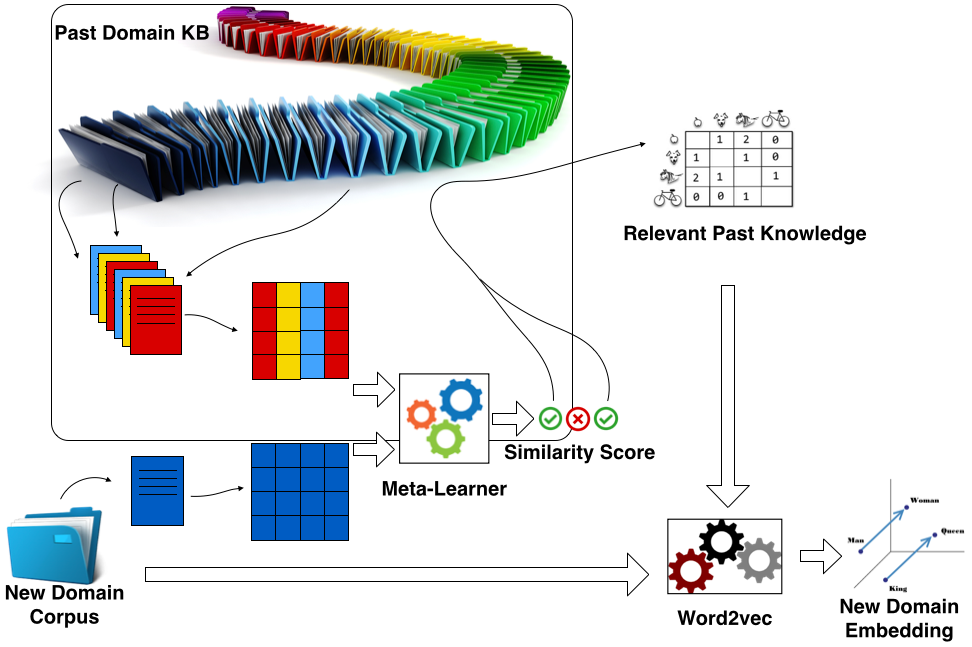
\includegraphics[width=5.0in]{fig/ijcai18_ll.png}
        \caption{Overview of L-DEM}
        \label{fig:fr}
    \end{figure}

\textbf{Base Meta-Learner}

This section describes the base meta-learner, which identifies similar domain contexts. The input to the meta-learner is a pair of word feature vectors (we simply call them \emph{feature vectors}) representing the domain contexts of the same word from two similar / non-similar domains.
The output of the meta-learner is a similarity score of the two feature vectors.

\textbf{Training Examples}

We assume the number of past domains is large and we hold out the first $m$ domains, where $m \ll n$, as the domains to train and test the base meta-learner.
In practice, if $n$ is small, the $m$ domains can be sampled from the $n$ domains.
The $m$ domains are split into 3 disjoint sets: training domains, validation domains, and testing domains.

To enable the meta-learner to predict the similarity score, we need both positive examples (from similar domains) and negative examples (from dissimilar domains).
Since each past domain can be unique (which makes it impossible to have a positive pair from two similar domains), we sub-sample each domain corpus $D_j$ into 2 sub-corpora: $D_{j, k} \sim P(D_i)$, where $1\le j\le m$ and $k=\{1, 2\}$.
This sampling process is done by drawing documents (each domain corpus is a set of documents) uniformly at random from $D_j$.
The number of documents that a domain sub-corpus can have is determined by a pre-defined sub-corpus (file) size.
We enforce the same file size across all sub-corpora so feature vectors from different sub-corpora are comparable.

Next, we produce feature vectors from domain sub-corpora.
Given a word $w_{i, j, k}$ (instance of the word $w_{i}$ in the domain sub-corpus $D_{j, k}$), we choose its co-occurrence counts on a fixed vocabulary $V_{\textit{wf}}$ within a context window (similar to word2vec) as the word $w_{i, j, k}$'s feature vector $\mathbf{x}_{w_{i, j, k}}$.
The fixed vocabulary $V_{\textit{wf}}$ (part of the KB used later, denoted as $\mathcal{K}.V_{\textit{wf}}$) is formed from the top-$f$ frequent words over $m$ domain corpora.
This is inspired by the fact that an easy-to-read dictionary (e.g., Longman dictionary) uses only a few thousand words to explain all words of a language.
A pair of feature vectors $(\mathbf{x}_{w_{i, j, k}}, \mathbf{x}_{w_{i, j, k'}})$ with $k \neq k'$, forms a postive example; 
whereas $(\mathbf{x}_{w_{i, j, k}}, \mathbf{x}_{w_{i, j', k}})$ with $j\neq j'$ forms a negative example.
Details of settings are in Section 6.

\textbf{Pairwise Model of the Meta-learner}

We train a small but efficient pairwise model (meta-learner) to learn a similarity score. 
Making the model small but high-throughput is crucial.
This is because the meta-learner is required in a high-throughput inference setting, where every word from a new domain needs to have context similarities with the same word from all past domains. 

The proposed pairwise model has only four layers. 
One shared fully-connected layer (with $l_1$-norm) is used to learn two continuous representations from two (discrete) input feature vectors.
A matching function is used to compute the representation of distance in a high-dimensional space.
Lastly, a fully-connected layer and a sigmoid layer are used to produce the similarity score.
The model is parameterized as follows:
\begin{equation}
\sigma \big( \bm{W}_2 \cdot \text{abs}\big( ( \bm{W}_1 \cdot \frac{\mathbf{x}_{w_{i, j, k}}}{ |\mathbf{x}_{w_{i, j, k}}|_1 }) - (\bm{W}_1 \cdot \frac{\mathbf{x}_{w_{i, j', k'}} }{ |\mathbf{x}_{w_{i, j', k'}}|_1 } ) \big) + b_2 \big) ,
\end{equation}
where $|\cdot|_1$ is the $l_1$-norm, $\text{abs}(\cdot)$ computes the absolute value of element-wise subtraction ($-$) as the matching function, $\bm{W}$s and $b$ are weights and $\sigma (\cdot)$ is the sigmoid function.
The majority of trainable weights resides in $\bm{W}_1$, which learns continuous features from the set of $f$ context words.
These weights can also be interpreted as a general embedding matrix over $V_{\textit{wf}}$. 
These embeddings (not related to the final domain embeddings in Chapter \ref{chap3:sec:aet}) help to learn the representation of domain-specific words.
As mentioned earlier, we train the base meta-learner $M$ over a hold-out set of $m$ domains.
We further fine-tune the base meta-learner using the new domain corpus for its domain use, as described in the next section.

\textbf{Embedding Using Past Relevant Knowledge}

We now describe how to leverage the base meta-learner $M$, the rest $n-m$ past domain corpora, and the new domain corpus $D_{n+1}$ to produce the new domain embeddings.

\textbf{Identifying Context Words from the Past}

When it comes to borrowing relevant knowledge from past domains, the first problem is what to borrow.
It is well-known that the embedding vector quality for a given word is determined by the quality and richness of that word's contexts.
We call a word in a domain context of a given word a \emph{context word}.
So for each word in the new domain corpus, we should borrow all context words from that word's similar domain contexts.
The algorithm for borrowing knowledge is described in Algorithm \ref{chap3:alg:ll}, which finds relevant past knowledge $\mathcal{A}$ (see below) based on the
knowledge base (KB) $\mathcal{K}$ and the new domain corpus $D_{n+1}$.

The KB $\mathcal{K}$ has the following pieces of information:
(1) the vocabulary of top-$f$ frequent words $\mathcal{K}.V_{\textit{wf}}$ (as discussed in Section 4.1), 
(2) the base meta-learner $\mathcal{K}.M$ (discussed in Section 4.2),
and (3) domain knowledge $\mathcal{K}_{m+1:n}$.
The domain knowledge has the following information:
(i) the vocabularies $V_{m+1:n}$ of past $n-m$ domains,
(ii) the sets of past word domain contexts $C_{m+1:n}$ from the past $n-m$ domains, where each $C_j$ is a set of key-value pairs $(w_{i,j}, \mathcal{C}_{w_{i,j} } )$ and $\mathcal{C}_{w_{i,j} } $ is a list of context words (We use list to simplify the explanation. In practice, bag-of-word representation should be used to save space.) for word $w_i$ in the $j$-th domain, 
and (iii) the sets of feature vectors $E_{m+1:n}$ of past $n-m$ domains, where each set $E_{j}=\{ \mathbf{x}_{w_{i, j, k}} | w_i \in V_{j} \text{ and } k=\{1, 2\} \}$.

The relevant past knowledge $\mathcal{A}$ of the new domain is the aggregation of all key-value pairs $(w_t, \mathcal{C}_{w_t})$, where $\mathcal{C}_{w_t}$ contains all similar domain contexts for $w_t$.

Algorithm \ref{chap3:alg:ll} retrieves the past domain knowledge in line 1.
Lines 2-4 prepare the new domain knowledge.
The BuildFeatureVector function produces a set of feature vectors as $E_{n+1}=\{ \mathbf{x}_{w_{i, n+1, k}} | w_i \in V_{j} \text{ and } k=\{1, 2\}\}$ over two sub-corpora of the new domain corpus $D_{n+1}$.
The ScanContextWord function builds a set of key-value pairs, where the key is a word from the new domain $w_{i, n+1}$ and the value $\mathcal{C}_{w_{i,n+1} } $ is a list of context words for the word $w_{i, n+1}$ from the new domain corpus. We use the same size of the context window as the word2vec model.

\textbf{Adapting Meta-learner}

In line 5, AdaptMeta-learner adapts or fine-tunes the base meta-learner $\mathcal{K}.M$ to produce an adapted meta-learner $M_{n+1}$ for the new domain.
A positive tuning example is sampled from two sub-corpora of the new domain $(\mathbf{x}_{w_{i, n+1, 1}}, \mathbf{x}_{w_{i, n+1, 2}})$.
A negative example is exampled as $(\mathbf{x}_{w_{i, n+1, 1}}, \mathbf{x}_{w_{i, j, 2}})$, where $m+1 \le j \le n$.
The initial weights of $M_{n+1}$ are set as the trained weights of the base meta-learner $M$. 
 
\begin{algorithm*}
\label{chap3:alg:ll}
\LinesNumbered
\DontPrintSemicolon
\caption{Identifying Context Words from the Past}
\SetKwInOut{Input}{Input} 
\SetKwInOut{Output}{Output} 
\SetKwRepeat{Do}{do}{while}
\Input{a knowledge base $\mathcal{K}$ containing a vocabulary $\mathcal{K}.V_{\textit{wf}}$, a base meta-learner $\mathcal{K}.M$, and domain knowledge $\mathcal{K}_{m+1:n}$; \\a new domain corpus $D_{n+1}$.}
\Output{relevant past knowledge $\mathcal{A}$, where each element is a key-value pair $(w_t, \mathcal{C}_{w_t})$ and $\mathcal{C}_{w_t}$ is a list of context words from all similar domain contexts for $w_t$. }
\BlankLine
\BlankLine
$(V_{m+1:n}, C_{m+1:n}, E_{m+1:n}) \gets \mathcal{K}_{m+1:n}$ \;
$V_{n+1} \gets \text{BuildVocab}(D_{n+1})$ \;
$C_{n+1} \gets \text{ScanContextWord}(D_{n+1}, V_{n+1})$ \;
$E_{n+1} \gets \text{BuildFeatureVector}(D_{n+1}, \mathcal{K}.V_{\textit{wf}})$ \;
$M_{n+1} \gets \text{AdaptMeta-learner}(\mathcal{K}.M, E_{m+1:n}, E_{n+1})$ \;
$\mathcal{A} \gets \emptyset$ \;

\For{$(V_j, C_j, E_j) \in (V_{m+1:n}, C_{m+1:n}, E_{m+1:n})$}{
    $O \gets V_j \cap V_{n+1}$  \;
    $F \gets \big\{(\mathbf{x}_{o, j, 1}, \mathbf{x}_{o, n+1, 1})|o \in O \text{ and } \mathbf{x}_{o, j, 1} \in E_j \text{ and } \mathbf{x}_{o, n+1, 1} \in E_{n+1} \big\}$ \;
    $S \gets M_{n+1}.\text{inference}( F )$ \;
    $O \gets \{o| o\in O \text{ and } S[o]\ge \delta \}$ \;
    \For{$o \in O$}{
        $\mathcal{A}[o].\text{append}(C_j[o] )$ \;
    }
}

$\mathcal{K}_{n+1} \gets (V_{n+1}, C_{n+1}, E_{n+1}) $ \;
\Return{ $\mathcal{A}$}
\end{algorithm*}

\textbf{Retriving Relevant Past Knowledge}

Algorithm \ref{chap3:alg:ll} further produces the relevant past knowledge $\mathcal{A}$ from line 6 through line 16.
Line 6 defines the variable that stores the relevant past knowledge.
Lines 7-15 produce the relevant past knowledge $\mathcal{A}$ from past domains.
The For block handles each past domain sequentially.
Line 8 computes the shared vocabulary $O$ between the new domain and the $j$-th past domain.
After retrieving the sets of feature vectors from the two domains in line 9, the adapted meta-learner uses its inference function (or model) to compute the similarity scores on pairs of feature vectors representing the same word from two domains (line 10).
The inference function can parallelize the computing of similarity scores in a high-throughput setting (e.g., GPU inference) to speed up.
Then we only keep the words from past domains with a score higher than a threshold $\delta$ at line 11.
Lines 12-14 aggregate the context words for each word in $O$ from past word domain contexts $C_j$.
Line 16 simply stores the new domain knowledge for future use.
Lastly, all relevant past knowledge $\mathcal{A}$ is returned.

\textbf{Augmented Embedding Training}
\label{chap3:sec:aet}

We now produce the new domain embeddings via a modified version of the skip-gram model \cite{mikolov2013distributed} that can take both the new domain corpus $D_{n+1}$ and the relevant past knowledge $\mathcal{A}$.
Given a new domain corpus $D_{n+1}$ with the vocabulary $V_{n+1}$, the goal of the skip-gram model is to learn a vector representation for each word $w_{i} \in V_{n+1}$ in that domain
(we omit the subscript $_{n+1}$ in $w_{i, n+1}$ for simplicity).
Assume the domain corpus is represented as a sequence of words $D_{n+1}=(w_1, \dots, w_T)$, the objective of the skip-gram model maximizes the following log-likelihood:
\begin{equation}
\label{chap3:eq:sg}
\begin{split}
\mathcal{L}_{D_{n+1}} =\sum_{t=1}^{T} \big( \sum_{w_c \in \mathcal{W}_{w_{t}} } \big(\log \sigma (\bm{u}_{w_t}^T\cdot \bm{v}_{w_c})
+ \sum_{w_{c'} \in \mathcal{N}_{w_t} } \log \sigma(-\bm{u}_{w_t}^T\cdot \bm{v}_{w_{c'}} ) \big) \big) , 
\end{split}
\end{equation}
where $\mathcal{W}_{w_t}$ is the set of words surrounding word $w_t$ in a fixed context window;
$\mathcal{N}_t$ is a set of words (negative samples) drawn from the vocabulary $V_{n+1}$ for the $t$-th word;
$\bm{u}$ and $\bm{v}$ are word vectors (or embeddings) we are trying to learn.
The objective of skip-gram on data of relevant past knowledge $\mathcal{A}$ is as follows:
\begin{equation}
\begin{split}
\mathcal{L}_{\mathcal{A}}=\sum_{(w_t, \mathcal{C}_{w_t} ) \in \mathcal{A}} \big( \sum_{w_c \in \mathcal{C}_{w_t}} \big( \log \sigma (\bm{u}_{w_t}^T\cdot \bm{v}_{w_c})
+ \sum_{w_{c'} \in \mathcal{N}_{w_t} } \log \sigma(-\bm{u}_{w_t}^T\cdot \bm{v}_{w_{c'}} ) \big) \big).
\end{split}
\end{equation}
Finally, we combine the above two objective functions as a single objective function:\\
\begin{equation}
\begin{split}
\mathcal{L}'_{D_{n+1}}=\mathcal{L}_{D_{n+1}} + \mathcal{L}_{\mathcal{A}}.
\end{split}
\end{equation}
We use the default hyperparameters of skip-gram model \cite{mikolov2013distributed} to train the domain embeddings.

\section{Results}
\label{chap3:sec:exp}

Following \cite{nayak2016evaluating},
we use the performances of down-stream tasks to evaluate the proposed method. 
We do not evaluate the learned embeddings directly as in \cite{mikolov2013distributed,pennington2014glove} because domain-specific dictionaries of similar / non-similar words are generally not available. Our down-stream tasks are text classification that usually requires fine-grained domain embeddings.

\textbf{Datasets}

We use the Amazon Review datasets from \cite{HeMcA16a}, which is a collection of multiple-domain corpora. We consider each second-level category (the first level is department) as a domain and aggregate all reviews under each category as one domain corpus. This ends up with a rather diverse domain collection. 
We first randomly select 56 ($m$) domains as the first $m$ past domains to train and evaluate the base meta-learner.
Then from rest domains, we sample three random collections with 50, 100 and 200 ($n-m$) domains corpora, respectively, as three settings of past domains.
These collections are used to test the performance of different numbers of past domains.
Due to the limited computing resource, we limit each past domain corpus up to 60 MB.
We further randomly selected 3 rest domains (\emph{Computer Components} (CC), \emph{Kitchen Storage and Organization} (KSO) and \emph{Cats Supply} (CS)) as new domains for down-stream tasks. These give us three text classification problems, which have 13, 17, and 11 classes respectively. The tasks are topic-based classification rather than sentiment classification. 
Since the past domains have different sizes (many have much less than 60 MB) and many real-world applications do not have big in-domain corpora, we set the size of the new domain corpora to be 10 MB and 30 MB to test the performance in the two settings.

\textbf{Evaluation of Meta-Learner}

We select the top $f=5000$ words from all 56 domains' corpora as word features.
Then we split the 56 domains into 39 domains for training, 5 domains for validation and 12 domains for testing.
So the validation and testing domain corpora have no overlap with the training domain corpora.
We sample 2 sub-corpora for each domain and limit the size of each sub-corpus to 10 MB. We randomly select 2000, 500, 1000 words from each training domain, validation domain, and testing domain, respectively, and ignore words with all-zero feature vectors to obtain pairwise examples. 
The testing 1000 words are randomly drawn and they have 30 overlapping words with the training 2000 words, but not from the same domains. So in most cases, it's testing the unseen words in unseen domains.
We set the size of a context window to be 5 when building feature vectors.
This ends up with 80484 training examples, 6234 validation examples, and 20740 test examples.
For comparison, we train an SVM model as a baseline.
The F1-score (for positive pairs) of SVM is 0.70, but the F1-score of the proposed base meta-learner model is \textbf{0.81}.

\begin{table}
\begin{center}

\begin{tabular}{l || c | c | c }
\hline
 & CC & KSO & CS\\
\hline
\hline
10MB & 0.832 & 0.841 & 0.856 \\
30MB & 0.847 & 0.859 & 0.876 \\
\hline

\end{tabular}
\caption{F1-score for L-DEM Meta-Learner}
%\caption{F1-score of positive predictions of the adapted meta-learner on 3 new domains: Computer Components (CC), Kitchen Storage and Organization (KSO) and Cats Supply (CS).}
\end{center}
\label{chap3:table:fine-tune}
\end{table}

To adapt the base meta-learner for each new domain. We sample 3000 words from each new domain, which results in slightly fewer than 6000 examples after ignoring all-zero feature vectors.
We select 3500 examples for training, 500 examples for validation and 2000 examples for testing.
The F1-scores on the test data are shown in Table 1.
Finally, we empirically set $\delta=0.7$ as the threshold on the similarity score in Algorithm \ref{chap3:alg:ll}, which roughly doubled the number of training examples from the new domain corpus. 
The size of the context window for building domain context is set to 5, which is the same as word2vec.

\begin{table}
\begin{center}

\scalebox{0.9}{

\begin{tabular}{l || c | c | c }
\hline
 & CC(13) & KSO(17) & CS(11)\\
\hline
\hline
NE  &  0.596  &  0.653  &  0.696 \\
fastText  &  0.705  &  0.717  &  0.809 \\
GoogleNews  &  0.76  &  0.722  &  0.814 \\
GloVe.Twitter.27B  &  0.696  &  0.707  &  0.80 \\
GloVe.6B  &  0.701  &  0.725  &  0.823 \\
GloVe.840B  &  0.803  &  0.758  &  0.855 \\
ND 10M  &  0.77  &  0.749  &  0.85 \\
ND 30M  &  0.794  &  0.766  &  0.87 \\
200D + ND 30M  &  0.795  &  0.765  &  0.859 \\
\hline
L-DENP 200D + ND 30M & 0.806 & 0.762 & 0.870 \\
\hline
L-DEM 200D + ND 10M  &  0.791  &  0.761  &  0.872 \\
L-DEM 50D + ND 30M  &  0.795  &  0.768  &  0.868 \\
L-DEM 100D + ND 30M  &  0.803  &  0.773  &  0.874 \\
L-DEM 200D + ND 30M  &  \textbf{0.809}  &  \textbf{0.775}  &  \textbf{0.883} \\
\hline

\end{tabular}
}
\caption{Accuracy of L-DEM}
%\caption{Accuracy of different embeddings on classification tasks for 3 new domains (numbers in parenthesis: the number of classes)}
\end{center}
\label{chap3:table:pc}
\end{table}

\textbf{Baselines and Our System}

Unless explicitly mentioned, the following embeddings have 300 dimensions, which are the same size as many pre-trained embeddings (GloVec.840B \cite{pennington2014glove} or fastText English Wiki\cite{bojanowski2016enriching}).\\
\textbf{No Embedding (NE)}: This baseline does not have any pre-trained word embeddings. The system randomly initializes the word vectors and train the word embedding layer during the training process of the downstream task.
\\
\textbf{fastText}: This baseline uses the lower-cased embeddings pre-trained from English Wikipedia using fastText \cite{bojanowski2016enriching}. We lower the cases of all corpora of down-stream tasks to match the words in this embedding. \\
\textbf{GoogleNews}: This baseline uses the pre-trained embeddings from word2vec (\url{https://code.google.com/archive/p/word2vec/} based on part of the Google News dataset, which contains 100 billion words.\\
\textbf{GloVe.Twitter.27B}: This embedding set is pre-trained using GloVe (\url{https://nlp.stanford.edu/projects/glove/}) based on Tweets of 27 billion words. This embedding is lower-cased and has 200 dimensions.\\
\textbf{GloVe.6B}: This is the lower-cased embeddings pre-trained from Wikipedia and Gigaword 5, which has 6 billion tokens. \\
\textbf{GloVe.840B}: This is the cased embeddings pre-trained from the Common Crawl corpus, which has 840 billion tokens.
This corpus contains almost all web pages available before 2015. 
We show that the embeddings produced from this very general corpus are sub-optimal for our domain-specific tasks.\\
\textbf{New Domain 10M (ND 10M)}: This is a baseline embedding pre-trained only from the new domain 10 MB corpus. 
We show that the embeddings trained from a small corpus alone are not good enough.\\
\textbf{New Domain 30M (ND 30M)}: This is a baseline embedding pre-trained only from the new domain 30 MB corpus. We increase the size of the new domain corpus to 30 MB to see the effect of the corpus size. \\
\textbf{200 Domains + New Domain 30M (200D + ND 30M)}: The embedding set trained by combining the corpora from all past 200 domains and the new domain. We use this baseline to show that using all past domain corpora may reduce the performance of the down-stream tasks. \\
\textbf{L-DENP 200D + ND 30M}: This is a \underline{N}on-\underline{P}arametric variant of the proposed method. We use TFIDF as the representation for a sentence in past domains and use cosine as a non-parametric function to compute the similarity with the TFIDF vector built from the new domain corpus. 
We report the results on a similarity threshold of 0.18, which is the best threshold ranging from 0.15 to 0.20.\\
\textbf{L-DEM Past Domains + New Domain (L-DEM [P]D + ND [X]M)}: These are different variations of our proposed method L-DEM. For example, ``L-DEM 200D + ND 30M'' denotes the embeddings trained from a 30MB new domain corpus and the relevant past knowledge from 200 past domains.

\textbf{Down-stream Tasks and Experiment Results}

As indicated earlier, we use classification tasks from 3 new domains (``Computer Components'', ``Cats Supply'' and ``Kitchen Storage and Organization'') to evaluate the embeddings produced by our system and compare them with those of baselines. 
These 3 new domains have 13, 17 and 11 classes (or product types), respectively.
For each task, we randomly draw 1500 reviews from each class to make up the experiment data, from which we keep 10000 reviews for testing (to make the result more accurate) and split the rest 7:1 for training and validation, respectively.
All tasks are evaluated on accuracy.
We train and evaluate each task on each system 10 times (with different initializations) and average the results.

For each task, we use an embedding layer to store the pre-trained embeddings.
We freeze the embedding layer during training, so the result is less affected by the rest of the model and the training data.
To make the performance of all tasks consistent, 
we apply the same Bi-LSTM model \cite{hochreiter1997long} on top of the embedding layer to learn task-specific features from different embeddings.
The input size of Bi-LSTM is the same as the embedding layer and the output size is 128.
All tasks use many-to-one Bi-LSTMs for classification purposes.
In the end, a fully-connected layer and a softmax layer are applied after Bi-LSTM, with the output size specific to the number of classes of each task.
We apply a dropout rate of 0.5 on all layers except the last one and use Adam \cite{kingma2014adam} as the optimizer.

Table 2 shows the main results. 
We observe that the proposed method L-DEM 200D + ND 30M performs the best.
The difference in the numbers of past domains indicates more past domains give better results.
The GloVe.840B trained on 840 billion tokens does not perform as well as embeddings produced by our method. 
GloVe.840B's performance on the CC domain is close to our method indicating mixed-domain embeddings for this domain are not bad and this domain is more general.  
Combining all past domain corpora with the new domain corpus (200D + ND 30M) makes the result worse than not using the past domains at all (ND 30M).
This is because the diverse 200 domains are not similar to the new domains.
The L-DENP 200D + ND 30M performs poorly indicating the proposed parametric meta-learner is useful, except the CC domain which is more general.

\section{Fusion of General and Domain Word Embeddings}
\label{chap3:sec:double}
%\subsection{-- Motivation}
The performance gain of domain word embeddings comes from the dense corpus focusing on a particular domain and the feature space dedicated to that particular domain. 
Although domain word embeddings are good at domain-specific features, many NLP tasks also require good features for general words that are unlikely to be affected by a particular domain too, such as those stop words.
As a result, those words are unlikely to be trained well due to the limited corpus of a particular domain, whereas general word embeddings have such an advantage by aggregating corpora from multiple domains together.
To the end, for a particular end task, how to leverage the benefits from both types of embeddings is essential for the success of an end task.  

\subsection{-- Approach}

One simple way is to concatenate the general word embeddings and domain-specific word embeddings.
Assume the input is a sequence of word indexes $\mathbf{x}=(x_1, \dots, x_n)$.
This sequence gets its two corresponding continuous representations $\mathbf{x}^g$ and $\mathbf{x}^d$ via two separate embedding layers (or embedding matrices) $W^g$ and $W^d$.
The first embedding matrix $W^g$ represents general embeddings pre-trained from a very large general-purpose corpus (usually hundreds of billions of tokens).
The second embedding matrix $W^d$ represents domain embeddings pre-trained from a small in-domain corpus, where the scope of the domain is exactly the domain that the training/testing data belongs to.

We do not allow these two embedding layers trainable because small training examples may lead to many unseen words in test data.
If embeddings are tunable, the features for seen words' embeddings will be adjusted (e.g., forgetting useless features and infusing new features that are related to the labels of the training examples).
%And the CNN filters will adjust to the new features accordingly. 
But the embeddings of unseen words from test data still have the old features that may be mistakenly extracted by future layers.
As such, we concatenate two embeddings $\mathbf{x}^{(1)}=\mathbf{x}^g \oplus \mathbf{x}^d$ and feed the hidden states to the rest layers of the network for the end task.

\subsection{-- Result}
We conducted experiments on two settings, one is in the same setting as for lifelong domain embeddings \cite{xumeta}; the other is for a sequence labeling task in sentiment analysis. We detail the architecture for aspect extraction later in Chapter \ref{chap6:sec:sa}.

\textbf{L-DEM for Text Classification}

\begin{table}
\begin{center}
\scalebox{0.80}{
\begin{tabular}{l || c | c | c }
\hline
 & CC(13) & KSO(17) & CS(11)\\
\hline
\hline
GloVe.840B\&ND 30M  &  0.811  &  0.78  &  0.885 \\
GloVe.840B\&L-DEM 200D+30M  &  \textbf{0.817}  &  \textbf{0.783}  &  \textbf{0.887} \\
\hline
\end{tabular}
}
\end{center}
\label{chap3:table:concat}
\caption{Concatenating Word Embeddings}
%\caption{Results of concatenated embeddings with GloVe.840B}
\end{table}

We evaluate two methods: (1) GloVe.840B\&ND 30M, which concatenates new domain only embeddings with GloVe.840B; (2) GloVe.840B\&L-DEM 200D + ND 30M, which concatenates our proposed embeddings with GloVe.840B. 
The results of concatenating general and domain-specific embeddings are shown in Chapter \ref{chap3:table:concat}.
Our method boosts the domain-specific parts of the embeddings further.
Note the ideal LL setting is to perform L-DEM on all domain corpora of the pre-trained embeddings.).

%Note that we did not compare with the existing transfer learning methods~\cite{bollegala2017think,bollegala-maehara-kawarabayashi:2015:ACL-IJCNLP,yang-lu-zheng:2017:EMNLP2017} as our approaches focus on domain-specific words in a lifelong learning setting, which do not need the user to provide the source domain(s) that are known to be similar to the target domain. 

%\section{Conclusions}
%In this paper, we formulated a domain word embedding learning process. 
%Given many previous domains and a new domain corpus, the proposed method can generate new domain embeddings by leveraging the knowledge in the past domain corpora via a meta-learner. 
%Experimental results show that our method is highly promising.

\chapter{Lifelong Contextualized Representation Learning}
\label{chap4:context}

Beyond word embeddings that only carry independent word-level features, the meaning (thus features or representations) of a word is also heavily affected by its contexts.
As a result, a good representation for an end task may not be only from a word embedding layer, but also from an encoder $E(x)$ that can consume a piece of text and provide representations for each word based on its nearby context in that sequence.
To learn such an encoder $E(x)$, researchers need to define a general proxy task that is close to almost all end tasks so to learn features for those end tasks.
The proxy task also needs to be self-supervised as the training corpora are unlabeled and can be as large as the corpus for word embeddings.

Language Model is a natural choice for such a proxy task, which aims to generate the rest texts given the input is corrupted from a piece of text.
Recent years of representation learning for NLP has a large focus on language models from large-scale unlabeled corpora, such as Elmo\cite{peters2018deep}, GPT/GPT2\cite{radford2018improving,radford2019language}, BERT\cite{devlin2018bert}, XLNet\cite{yang2019xlnet}, RoBERTa\cite{liu2019roberta}, ALBERT\cite{lan2019albert}, ELECTRA\cite{clark2019electra}.
The idea behind the progress is that even though the word embedding \cite{mikolov2013distributed,pennington2014glove} layer (in a typical neural network for NLP) is trained from large-scale corpora, training a wide variety of neural architectures that encode contextual representations only from the limited supervised data on end tasks is insufficient.

BERT\cite{devlin2018bert} is one of the key innovations in the recent progress.
The magic behind BERT is the proposed proxy task of masked language model(MLM), which does not aim to generate the next token from the previous token but randomly masking out a portion of tokens from a whole text and task the model to predict.
The key benefit of MLM is that it enables a more complex reasoning process of learning and reasoning from the corrupted (masked) input that not only learns from a unidirectional context (e.g., left side of the current token) but from bidirectional contexts.
This naturally ended with more deeper reasoning and general features from contexts rather than hard-coded features from a particular piece of text.

\section{Motivation}
\label{chap4:sec:motivation}

Although BERT aims to learn contextualized representations across a wide range of NLP tasks (to be task-agnostic), leveraging BERT alone still leaves the domain challenges unresolved (as BERT is trained on Wikipedia articles and has almost no understanding of the text on a particular domain).
As such, BERT only learns features for text in general but largely ignores knowledge for a particular domain.
Also, since BERT aims to learn features for almost all end tasks, it introduces another challenge of task-awareness, called the \textit{task challenge}.
This challenge arises when the task-agnostic BERT meets the limited number of fine-tuning examples in end tasks, which is insufficient to fine-tune BERT to ensure full task-awareness of the system.
For example, the end tasks from the original BERT paper typically use tens of thousands of examples to ensure that the system is task-aware.
Inspired by these observations, I introduce a lifelong learning style of training.

\section{Lifelong Training}

To address the challenges, I propose a lifelong learning style training by introducing extra training tasks within the well-known pre-training and fine-tuning framework.
I explore two (2) training task (or step) into the existing framework: post-training and pre-tuning, as depicted in \ref{chap4:fig:ll_train}.

\begin{figure}
\centering
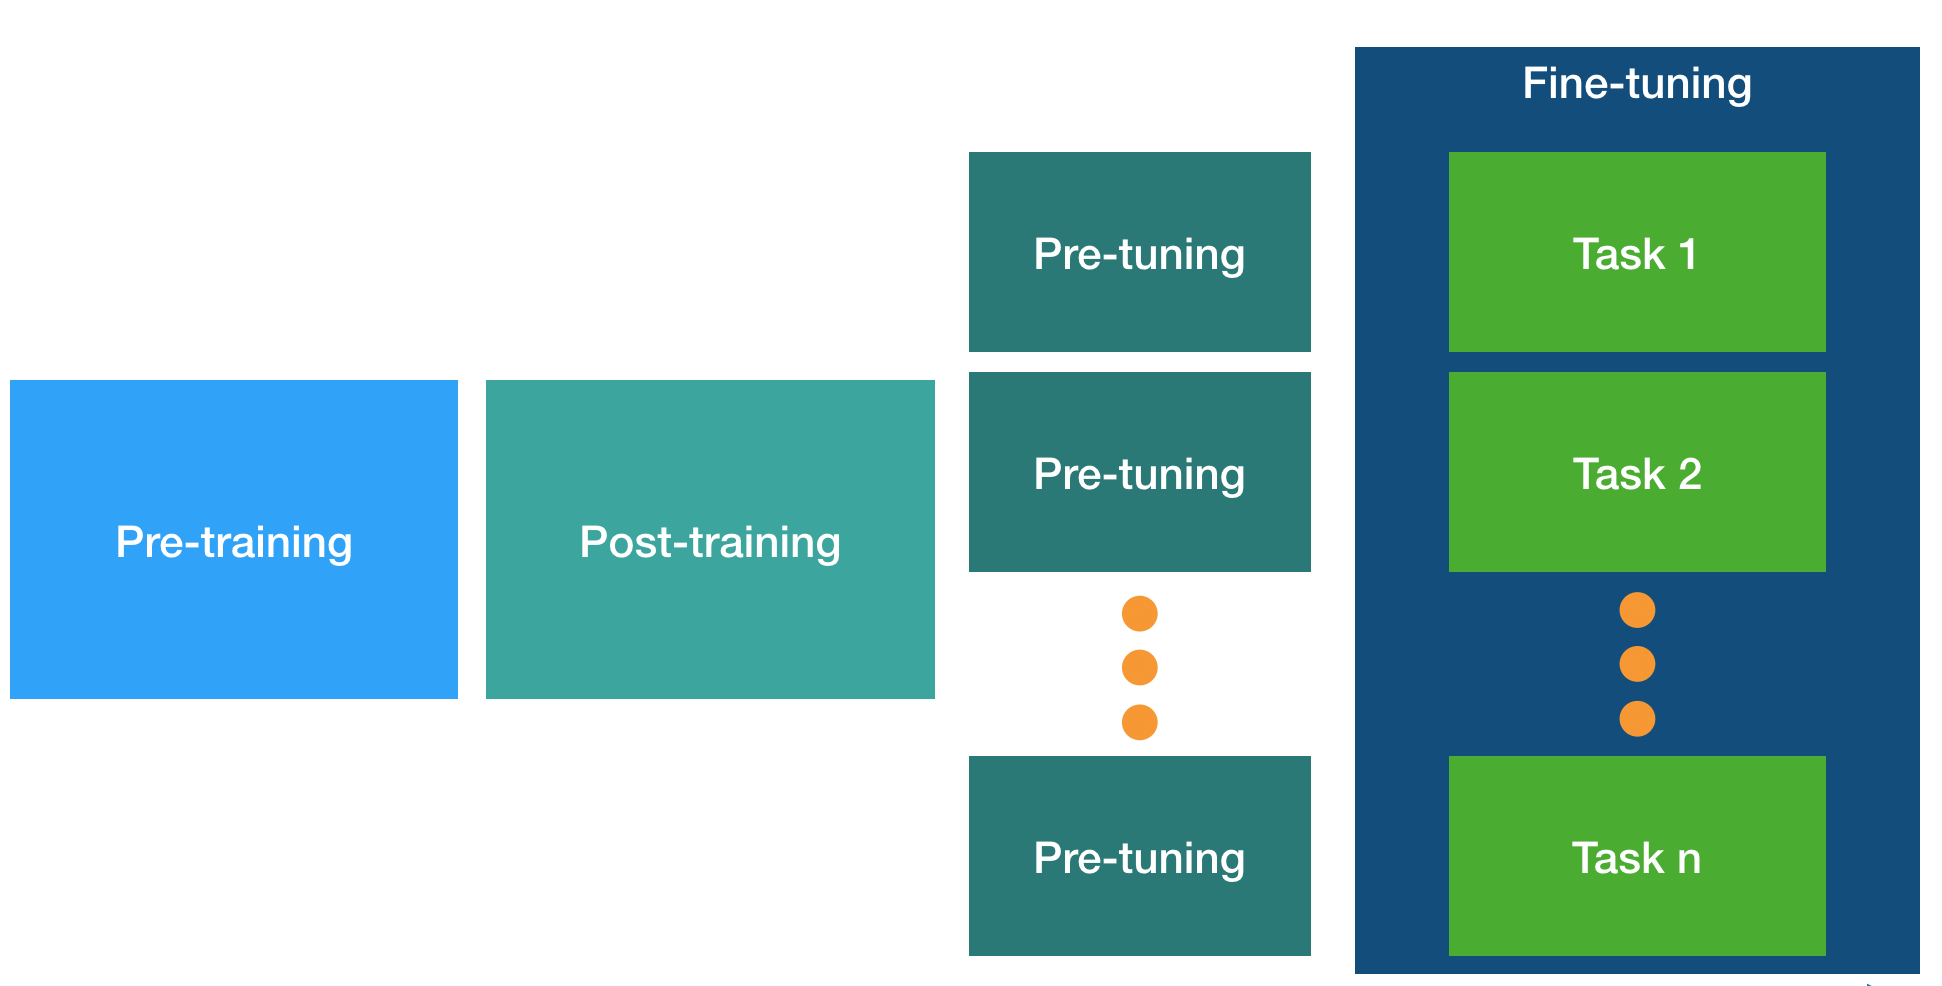
\includegraphics[width=5.5in]{fig/ll_train.png}
    \caption{Lifelong stages of training}
\label{chap4:fig:ll_train}
\vspace{-3mm}
\end{figure}

Post-training aims to adapt pre-training LM from general text to domain-specific text, whereas pre-tuning aims to adapt pre-trained LM to a particular task.

\subsection{-- Post-training of Language Models}
\label{chap4:sec:post-training}

I propose a novel joint post-training technique that takes BERT's pre-trained weights as the initialization (Due to limited computation resources, it is impractical for us to pre-train BERT directly on reviews from scratch \cite{devlin2018bert}.) for basic language understanding and adapts BERT with domain knowledge.
I also incorporate tasks from a supervised learning corpus from a machine reading comprehension task (MRC) that carries high-quality QA knowledge annotated by humans.
Results show that this task further improves the learned representation.
As a result, post-training leverages knowledge from two sources: unsupervised domain reviews and supervised (yet out-of-domain) MRC data.

BERT has two parameter intensive settings:\\
\noindent
$\textbf{BERT}_\textbf{BASE}$: 12 layers, 768 hidden dimensions and 12 attention heads (in transformer) with the total number of parameters, 110M;\\
\noindent
$\textbf{BERT}_\textbf{LARGE}$: 24 layers, 1024 hidden dimensions and 16 attention heads (in transformer) with the total number of parameters, 340M.

%As discussed in the introduction, fine-tuning BERT directly on the end task that has limited tuning data faces both domain challenges and task-awareness challenge.
%To enhance the performance of RRC (and also AE and ASC), we may need to reduce the bias introduced by non-review knowledge (e.g., from Wikipedia corpora) and fuse domain knowledge (DK) (from unsupervised domain data) and task knowledge (from supervised MRC task but out-of-domain data).
%Given MRC is a general task with answers of questions covering almost all document contents, a large-scale MRC supervised corpus may also benefit AE and ASC.
%Eventually, we aim to have a general-purpose post-training strategy that can exploit the above two kinds of knowledge for end tasks.

To post-train on domain knowledge, we leverage the two novel pre-training objectives from BERT: masked language model (MLM) and next sentence (The BERT paper refers a sentence as a piece of text with one or more natural language sentences.) prediction (NSP). The former predicts randomly masked words and the latter detects whether two sides of the input are from the same document or not.~A training example is formulated as $(\texttt{[CLS]}, x_{1:j}, \texttt{[SEP]}, x_{j+1:n}, \texttt{[SEP]})$, where $x_{1:n}$ is a document (with randomly masked words) split into two sides $x_{1:j}$ and $x_{j+1:n}$ and \texttt{[SEP]} separates those two.

MLM is crucial for injecting review domain knowledge and for alleviating the bias of the knowledge from Wikipedia. 
For example, in the Wikipedia domain, BERT may learn to guess the \texttt{[MASK]} in ``The \texttt{[MASK]} is bright'' as ``sun''. But in a laptop domain, it could be ``screen''.
Further, if the \texttt{[MASK]}ed word is an opinion word in ``The touch screen is \texttt{[MASK]}'', this objective challenges BERT to learn the representations for fine-grained opinion words like ``great'' or ``terrible'' for \texttt{[MASK]}.
The objective of NSP further encourages BERT to learn contextual representation beyond word-level.
In the context of reviews, NSP formulates a task of ``artificial review prediction'', where a negative example is an original review but a positive example is a synthesized fake review by combining two different reviews.
This task exploits the rich relationships between two sides in the input, such as whether two sides of texts have the same rating or not (when two reviews with different ratings are combined as a positive example), or whether two sides are targeting the same product or not (when two reviews from different products are merged as a positive example).
In summary, these two objectives encourage to learn a myriad of fine-grained features for potential end tasks. 

We let the loss function of MLM be $\mathcal{L}_{\text{MLM}}$ and the loss function of next text piece prediction be $\mathcal{L}_{\text{NSP}}$, the total loss of the domain knowledge post-training is $\mathcal{L}_{\text{DK}}=\mathcal{L}_{\text{MLM}} + \mathcal{L}_{\text{NSP}} $.

To post-train BERT on general QA knowledge, we use SQuAD (1.1), which is a popular large-scale MRC dataset.

We let the loss on SQuAD be $\mathcal{L}_{\text{MRC}}$, which is in a similar setting as the loss $\mathcal{L}_{\text{RRC}}$ for RRC.
As a result, the joint loss of post-training is defined as $\mathcal{L}=\mathcal{L}_{\text{DK}} + \mathcal{L}_{\text{MRC}}$.

One major issue of post-training on such a loss is the prohibitive cost of GPU memory usage.
Instead of updating parameters over a batch, we divide a batch into multiple sub-batches and accumulate gradients on those sub-batches before parameter updates. This allows for a smaller sub-batch to be consumed in each iteration.

\begin{algorithm}[t]
\label{chap4:alg:post-training}
\LinesNumbered
\DontPrintSemicolon
\caption{Post-training Algorithm}
\SetKwInOut{Input}{Input} 
\Input{$\mathcal{D}_\text{DK}$: one batch of DK data; \\$\mathcal{D}_\text{MRC}$ one batch of MRC data; \\$u$: number of sub-batches.}
\BlankLine
$\nabla_\Theta \mathcal{L} \gets 0 $ \;
$\{\mathcal{D}_{\text{DK}, 1}, \dots, \mathcal{D}_{\text{DK}, u} \} \gets \text{Split}(\mathcal{D}_\text{DK}, u) $ \;
$\{\mathcal{D}_{\text{MRC}, 1}, \dots, \mathcal{D}_{\text{MRC}, u} \} \gets \text{Split}(\mathcal{D}_\text{MRC}, u) $ \;
\For{$i \in \{1, \dots, u\}$ }{
    $\mathcal{L}_\text{partial}\gets \frac{\mathcal{L}_{\text{DK}}(\mathcal{D}_{\text{DK}, i}) + \mathcal{L}_{\text{MRC}}(\mathcal{D}_{\text{MRC}, i} )}{u} $ \;
    $\nabla_\Theta \mathcal{L} \gets \nabla_\Theta \mathcal{L} + \text{BackProp}(\mathcal{L}_\text{partial}) $\;
}
$\Theta \gets \text{ParameterUpdates}(\nabla_\Theta \mathcal{L}) $ \;
\end{algorithm}

Algorithm 1 describes one training step and takes one batch of data on domain knowledge (DK) $\mathcal{D}_\text{DK}$ and one batch of MRC training data $\mathcal{D}_\text{MRC}$ to update the parameters $\Theta$ of BERT.
In line 1, it first initializes the gradients $\nabla_\Theta$ of all parameters as 0 to prepare gradient computation. Then in lines 2 and 3, each batch of training data is split into $u$ sub-batches. Lines 4-7 spread the calculation of gradients to $u$ iterations, where the data from each iteration of sub-batches are supposed to be able to fit into GPU memory.
In line 5, it computes the partial joint loss $\mathcal{L}_\text{partial}$ of two sub-batches $\mathcal{D}_{\text{DK}, i}$ and $\mathcal{D}_{\text{MRC}, i}$ from the $i$-th iteration through forward pass.
Note that the summation of two sub-batches' losses is divided by $u$, which compensates the scale change introduced by gradient accumulation in line 6.
Line 6 accumulates the gradients produced by backpropagation from the partial joint loss. To this end, accumulating the gradients $u$ times is equivalent to computing the gradients on the whole batch once. But the sub-batches and their intermediate hidden representations during the $i$-th forward pass can be discarded to save memory space.
Only the gradients $\nabla_\Theta$ are kept throughout all iterations and used to update parameters (based on the chosen optimizer) in line 8.
%We detail the hyper-parameter settings of this algorithm in Sec. %\ref{chap4:sec:hyp}.

\textbf{Setting for End Tasks}

We aim for 3 review-based tasks to evaluate the post-trained BERT: review reading comprehension (RRC), aspect extraction (AE) and aspect sentiment classification (ASC).
The details of these 3 tasks are intoduced in \ref{chap6:nlp}.
Here we only discuss the formulation of these 3 tasks under the setting of BERT.
The overall illustrations of the formulation are depicted in \ref{chap6:fig:overview}.

\begin{figure}
\centering
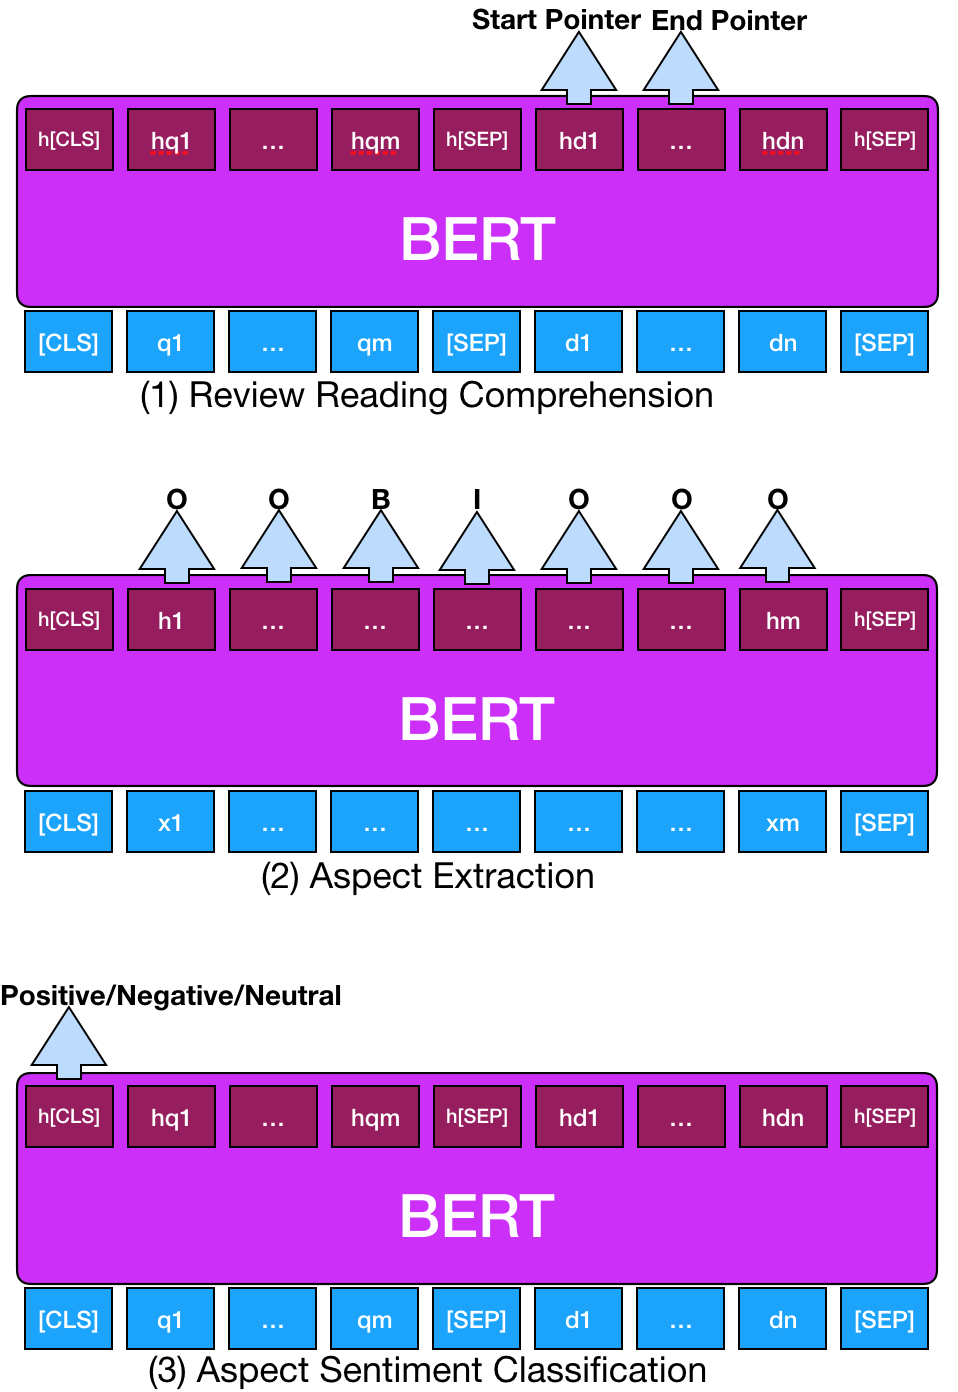
\includegraphics[width=5.5in]{fig/naacl19_overview.png}
    \caption{BERT for end tasks}
\label{chap6:fig:overview}
\vspace{-3mm}
\end{figure}

Following the success of SQuAD \cite{rajpurkar2016squad} and BERT's SQuAD implementation, we design review reading comprehension as follows.
Given a question $q=(q_1, \dots, q_m)$ asking for an answer from a review $d=(d_1, \dots, d_n)$, we formulate the input as a sequence $x=(\texttt{[CLS]}, q_1, \dots, q_m, \texttt{[SEP]}, d_1, \\ \dots, d_n, \texttt{[SEP]})$, where \texttt{[CLS]} is a dummy token not used for RRC and \texttt{[SEP]} is intended to separate $q$ and $d$.
Let $\text{BERT}(\cdot)$ be the pre-trained (or post-trained as in the next section) BERT model. We first obtain the hidden representation as $h=\text{BERT}(x) \in \mathbb{R}^{r_h*|x|}$, where $|x|$ is the length of the input sequence and $r_h$ is the size of the hidden dimension. Then the hidden representation is passed to two separate dense layers followed by softmax functions: $l_1=\text{softmax}(W_1 \cdot h + b_1)$ and $l_2=\text{softmax}(W_2 \cdot h + b_2)$, where $W_1$, $W_2 \in \mathbb{R}^{r_h}$ and $b_1, b_2 \in \mathbb{R}$. The \text{softmax} is applied along the dimension of the sequence.
The output is a span across the positions in $d$ (after the \texttt{[SEP]} token of the input), indicated by two pointers (indexes) $s$ and $e$ computed from $l_1$ and $l_2$: $s=\argmax_{ \text{Idx}_{\texttt{[SEP]}} < s<|x|}(l_1)$ and $e=\argmax_{s\le e<|x|}(l_2)$, where $\text{Idx}_{\texttt{[SEP]}}$ is the position of token \texttt{[SEP]} (so the pointers will never point to tokens from the question).
As such, the final answer will always be a valid text span from the review as $a=(d_s, \dots, d_e)$.

Training the RRC model involves minimizing the loss that is designed as the averaged cross entropy on the two pointers: $$\mathcal{L}_{\text{RRC}}=-\frac{\sum \log l_1 \mathbb{I}(s)+ \sum \log l_2 \mathbb{I}(e)}{2},$$ where $\mathbb{I}(s)$ and $\mathbb{I}(e)$ are one-hot vectors representing the ground truths of pointers.

As a core task in ABSA, aspect extraction (AE) aims to find aspects that reviewers have expressed opinions on \cite{hu2004mining}. 
In supervised settings, it is typically modeled as a sequence labeling task, where each token from a sentence is labeled as one of $\{\textit{\underline{B}egin}, \textit{\underline{I}nside}, \textit{\underline{O}utside}\}$. A continuous chunk of tokens that are labeled as one \textit{B} and followed by zero or more \textit{I}s forms an aspect.
The input sentence with $m$ words is constructed as $x=(\texttt{[CLS]}, x_1, \dots, x_m, \texttt{[SEP]})$.
After $h=\text{BERT}(x)$, we apply a dense layer and a softmax for each position of the sequence: $l_3=\text{softmax}(W_3 \cdot h + b_3)$, where $W_3 \in \mathbb{R}^{3*r_h}$ and $b_3 \in \mathbb{R}^3$ (3 is the total number of labels (\textit{BIO})).  Softmax is applied along the dimension of labels for each position and $l_3 \in [0, 1]^{3*|x|}$. The labels are predicted as taking argmax function at each position of $l_3$ and the loss function is the averaged cross entropy across all positions of a sequence.

As a subsequent task of AE, aspect sentiment classification (ASC) aims to classify the sentiment polarity (positive, negative, or neutral) expressed on an aspect extracted from a review sentence.
There are two inputs to ASC: an aspect and a review sentence mentioning that aspect.

Let $x=(\texttt{[CLS]}, q_1, \dots, q_m, \texttt{[SEP]}, d_1, \dots, d_n, \texttt{[SEP]})$, where $q_1, \dots, q_m$ now is an aspect (with $m$ tokens) and $d_1, \dots, d_n$ is a review sentence containing that aspect.
After $h=\text{BERT}(x)$, we leverage the representations of \texttt{[CLS]} $h_{\text{[CLS]}}$, which is the aspect-aware representation of the whole input.
The distribution of polarity is predicted as $l_4=\text{softmax}(W_4 \cdot h_{\text{[CLS]}} + b_4)$, where $W_4 \in \mathbb{R}^{3*r_h}$ and $b_4 \in \mathbb{R}^3$ (3 is the number of polarities). Softmax is applied along the dimension of labels on \texttt{[CLS]}: $l_4 \in [0, 1]^{3}$.
Training loss is the cross-entropy on the polarities.

As a summary of these tasks, insufficient supervised training data significantly limits the performance gain across these 3 review-based tasks.~Although BERT's pre-trained weights strongly boost the performance of many other NLP tasks on formal texts, we observe in Chapter \ref{chap6:sec:exp} that BERT's weights only result in a limited gain or worse performance compared with existing baselines.

\textbf{Post-training datasets}

For domain knowledge post-training, we use Amazon laptop reviews \cite{HeMcA16a} and Yelp Dataset Challenge reviews (\url{https://www.yelp.com/dataset/challenge}).
For laptop domain, we filtered out reviewed products that have appeared in the validation/test reviews to avoid training bias for test data (Yelp reviews do not have this issue as the source reviews of SemEval are not from Yelp). 
Since the number of reviews is small, we choose a duplicate factor of 5 (each review generates about 5 training examples) during BERT data pre-processing.
This gives us 
1,151,863 post-training examples for laptop domain knowledge.

For the restaurant domain, we use Yelp reviews from restaurant categories that the SemEval reviews also belong to \cite{xu_acl2018}.
We choose 700K reviews to ensure it is large enough to generate training examples (with a duplicate factor of 1) to cover all post-training steps that we can afford (discussed in Section 
%\ref{chap4:sec:hyp}
) (We expect that using more reviews can have even better results but we limit the number of reviews based on our computational power.).
This gives us 2,677,025 post-training examples for restaurant domain knowledge learning.

For general RC knowledge, we leverage SQuAD 1.1 \cite{rajpurkar2016squad} that comes with 87,599 training examples from 442 Wikipedia articles.
The experiments are discussed in Chapter \ref{chap6:nlp} when addressing each specific task.

\subsection{-- Pre-tuning for End-tasks}
\label{chap4:sec:pre-tuning}

Different from post-training that aims for domain adaption, pre-tuning is preparing a pre-trained (or even post-trained) model for a particular end-task.
Pre-tuning is proposed to improve the performance of potential end tasks that are limited by training data.
Although BERT is successful on many end tasks, those end tasks typically have thousands of training data.
In real-world settings of machine learning, it is often the case humans have limited power to provide enough training data for each end task.
This makes the proposed pre-tuning very important because the pre-training stage is targeting a general proxy task, not one particular end task, which leads to a large discrepancy or gap between the pre-training and fine-tuning task.
This is especially true when the masked language model aims to guess the correct tokens for $\texttt{[MASK]}$s, which are never appear in an end task.

Beyond that, many NLP tasks have more complex formats than the format of MLM (or next sentence prediction (NSP) if the proxy task has that).
This difference yields an even larger discrepancy that a limited training data for an end task cannot fine-tune the pre-trained model enough.
In my research on pre-tuning, I give a task called review conversational reading comprehension (RCRC), which needs to carry multiple past turns of question answering as input to the model that does not appear in the pre-training stage of BERT.
We define the textual format of RCRC in the following way and form a pre-tuning task to improve the supervised learning from limited end task data.

\textbf{Textual Format}
\label{chap4:sec:format}

Inspired by the DrQA system \cite{reddy2018coqa}, we formulate an input example $x$ for both RCRC fine-tuning and pre-tuning (We share the same notation for both tasks for brevity.) as a composition of the context $C$, the current question $q_k$, and a review $d$:
\vspace*{-2mm}
\begin{equation}
\begin{split}
(\texttt{[CLS]} \texttt{[Q]} q_1 \texttt{[A]} a_1 \dots \texttt{[Q]} q_{k-1} \texttt{[A]} a_{k-1} \texttt{[Q]} q_{k} \texttt{[SEP]} d_{1:n} \texttt{[SEP]}),
\nonumber
\end{split}
\vspace*{-5mm}
\end{equation}
where past QA pairs $q_1, a_1, \dots, q_{k-1}, a_{k-1}$ in $C$ are concatenated and separated by two tokens \texttt{[Q]} and \texttt{[A]} and then concatenated with the current question $q_k$ as the left side of BERT and the right side is the review document.
One can observe that BERT lacks the basic understanding of the RCRC task regarding both the input and output, such as the above input format and textual spans in a review. Limited training data of $(\text{RC})_2$ may not be sufficient to learn such a complex input and output.
We propose a pre-tuning stage that can enhance the understanding of the input/output before fine-tuning on $(\text{RC})_2$.

\textbf{Data Formulation for Pre-tuning}
\label{chap4:sec:form}

We first formulate the data for pre-tuning that aims to address the understanding of the textual format.
As we have no annotated data except the limited $(\text{RC})_2$ data, we harvest domain QA pairs and reviews, which are typically organized under an entity (a laptop or a restaurant). The QA pairs and reviews are combined to produce the pre-tuning examples. The process is given in Algorithm \ref{chap4:alg:pre-tuning}.

\begin{algorithm}[t]
    \label{chap4:alg:pre-tuning}
    \LinesNumbered
    \DontPrintSemicolon
    \caption{Data Generation Algorithm}
    \SetKwInOut{Input}{Input} 
    \SetKwInOut{Output}{Output} 
    \Input{$\mathcal{Q}$: a set of QA pairs; $\mathcal{R}$: a set of reviews; $h_{max}$: maximum turns in context.}
    \Output{$\mathcal{T}$: pre-tuning data.}

    \BlankLine

    $\mathcal{T} \gets \{\}$ \;
    \For{$(q', a') \in \mathcal{Q}$ }{
        $x \gets \texttt{[CLS]} $ \;
        $h \gets \text{RandInteger}([0, h_{\text{max}}]) $ \;
        \For{$1 \to h$}{
            $q'', a'' \gets \text{RandSelect}(\mathcal{Q}\backslash(q', a'))$ \;
            $ x \gets x \oplus \texttt{[Q]} \oplus q'' \oplus \texttt{[A]} \oplus a'' $\;
        }
        $ x \gets x \oplus \texttt{[Q]} \oplus q' \texttt{[SEP]} $ \;
        $ r_{1:m} \gets \text{RandSelect}(\mathcal{R}) $ \;
        \If{$\text{RandFloat}([0.0, 1.0]) > 0.5$ }{
            $(\_, a) \gets \text{RandSelect}(\mathcal{Q}\backslash(q', a') ) $ \;
            $(u, v) \gets (1, 1)$ \;
        }
        \Else{$a \gets a'$ \;
            $(u, v) \gets (|x|, |x|+|a|) $ \;
        }
        $ l \gets \text{RandInteger}([0, u]) $ \;
        $ d_{1:n} \gets r_{0:l} \oplus a \oplus r_{l+1:u} $ \;
        \If{$u>1$ }{
            $ (u, v) \gets (u+|r_{0:l}|, v+|r_{0:l}|) $
        }
        $x \gets x \oplus d_{1:n} \oplus \texttt{[SEP]}$ \;
        $\mathcal{T} \gets \mathcal{T} + (x, (u, v) )$ \;
    }
\end{algorithm}

The inputs to Algorithm \ref{chap4:alg:pre-tuning} are a set of QA pairs and a set of reviews belonging to the same entity and the maximum number of turns in the context. The output is the pre-tuning data, which is initialized in Line 1. 
Each example is denoted as $(x, (u, v))$, where $x$ is the input example and $(u, v)$ indicates the boundary (starting and ending indexes) of an answer for the auxiliary objective (discussed in the next section).
Given a QA pair $(q', a')$ in Line 2, we first build the left side of input example $x$ in Line 3-9.
After initializing input $x$ in Line 3, we randomly determine the number of turns in the context in Line 4 and concatenate $\oplus$ these turns of QA pairs in Line 5-8, where $\mathcal{Q}\backslash(q', a')$ ensures the current QA pair $(q', a')$ is not chosen.
In Line 9, we concatenate with the current question $q'$.
Lines 10-23 build the right side of input example $x$ and the answer boundary.
In Line 10, we randomly draw a review of $r$ with $m$ sentences. To challenge the pre-tuning stage to discover the semantic relatedness between $q'$ and $a'$ (for the auxiliary objective), we first decide whether to allow the right side of $x$ contains $a'$ (Line 16) for $q'$ or a random (negative/no) answer $a$ in Lines 11-12.
We also come up with two indexes $u$ and $v$ initialized in Lines 13 and 17.
Then, we insert $a$ into review $r$ by randomly picking one from the $m+1$ locations in Lines 19-20.
This gives us $d_{1:n}$, which has $n$ tokens. 
We further update $u$ and $v$ to allow them to point to the chunk boundaries of $a'$.
Otherwise, BERT should detect no $a'$ on the right side and point to \texttt{[CLS]} ($u,v=1$). Finally, examples are aggregated in Line 25.
Algorithm \ref{chap4:alg:pre-tuning} is run $k$ times to allow for enough samplings. 
Following BERT, we still randomly mask some words in each example $x$ but omitted here for brevity.

\textbf{Auxilary Objective}
\label{chap4:sec:aux}

Besides the input, we further adapt BERT to the output of RCRC with an auxiliary objective.
The design of this auxiliary objective is to mimic a prediction of a textual span in RCRC, which aims to predict the token spans of an answer randomly inserted in the review or \textit{NO ANSWER} if a randomly drawn negative answer appears.
The implementation of both the auxiliary objective and the RCRC model is similar to BERT for SQuAD 2.0 \cite{rajpurkar2018know}, so we omit them for brevity.
After pre-tuning, we fine-tune using the $(\text{RC})_2$ dataset to show the performance of RCRC.
The results of RCRC is discussed in \ref{chap6:sec:rcrc}.


\chapter{Lifelong Graph Representation Learning}
\label{chap5:graph}

Besides classification and word representations that aims to turn unstructured text into a structured form, knowledge graph is an important form of structured data that possess human knowledge.
Different from unstructured text, knowledge graph is more interpretable and maintainable by human.
Given the discrete nature of the knowledge graph, it enables the dynamic accumulation of structured knowledge for future use, which is the goal of lifelong learning.
In this setting, one task in lifelong learning can contribute to the updates of a knowledge graph and the future task can leverage the updated knowledge graph for better reasoning or prediction.
Thus, I target a lifelong graph representation learning task, where the model should learn representations for the changes of knowledge graph for better reasoning or prediction.

\section{Motivation}

Existing research on the knowledge graph mostly assumes a static graph.
This is because they assume a (factoid) knowledge graph, where knowledge inside is rather stable and seldom change.
This is true for most factoid-based knowledge in the world.
The changes of the knowledge mostly happen when new events happen and engineers can periodically add new entity or relation to the knowledge graph when enough statistics of data are collected for more reliable updates of knowledge.

However, in contrast, non-factoid knowledge is rather dynamic and needs more updates.
Non-factoid knowledge can be that knowledge that does not have agreement among a group of people, but particular to one or a small group of people.
There is probably no true or false regarding these kinds of knowledge.
These include the experience of a user and their preference or sentiment.
This kind of knowledge is rather unstable because even the same person can change their mind quickly and a lifelong learning system should be able to capture such changes quickly.

One important application regarding this kind of knowledge is a recommendation, as almost all recommendation models are user-specific models, which have different predictions for different users.
Typically these models aim to learn users and items profile, such as using matrix factorization based on click-through data.
Unfortunately, existing recommendation models aim to learn static user and item profiles.
These static profiles cannot capture the changes in users' needs.
As such, conversational recommendation \cite{li2018towards,kang2019recommendation} is a novel type of task that allows using an interactive dialog to collect users' up-to-date preference to update the user profile.
Although existing research in conversational recommendation aims to update the user profile in the hidden space, modeling users' profile as a knowledge graph has the following two (2) benefits: (1) it allows for easier updates and maintenance of user profile for long-term use given the semantics of the hidden space is mostly undefined and determined by random initialization; (2) it allows for interpretability given the discrete structure of knowledge graph.

To this end, a user's profile can be ideally represented as a knowledge graph, which requires frequent updates, even in one turn of a dialog between the AI agent and a user.
More importantly, I aim to design a universal knowledge graph that contains almost all knowledge in a recommendation setting, including information from both the users and items.
As such, this chapter focuses on designing and maintaining a knowledge graph for recommendation under a conversation setting, where the representation of the knowledge graph needs to be updated frequently for reasoning a better dialog policy.

\section{Lifelong Knowledge Graph Reasoning}
\label{chap5:sec:reason}

As an example of lifelong representation learning over a dynamic knowledge graph, we demonstrate the usage of dynamic knowledge graph reasoning with an application in dialog system. 
This task is called conversational recommendation. 
Conversational recommendation is a combination of dialog system and recommender system and aims to collect a user's up-to-date knowledge for recommendation. 
We focus on the graph maintanance aspect of conversational recommendation in this chapter and  detail the application side of this task in Chapter \ref{chap6:sec:mgcr}.
We call the knowledge graph about a user memory because it is the agent's memory about a user.
 
\textbf{Memory-grounded Conversational Recommendation}:
Given the history of previous items $\mathcal{H}$ (interacted or visited, etc.), candidate items $\mathcal{C}$ for recommendation, and their attributes (values), 
an agent first (1) constructs a user memory graph $\mathcal{G} = \{(e, r, e')\vert e, e' \in \mathcal{E}, r \in \mathcal{R} \}$ for user $e_u$; 
then (2) for each turn $d \in D$ of a dialog, the agent updates $\mathcal{G}$ with tuples of preference $\mathcal{G}' \gets \mathcal{G} \cup \{(e_u, r_1, e_1), \dots\}$ ;
(3) performs reasoning over $\mathcal{G}'$ to yield a dialog policy $\pi$ that
either (i) performs more rounds of interaction by asking for more preference, 
or (ii) predicts optimal (or ground truth) items for recommendations $\mathcal{T} \subset \mathcal{C}$.

\textbf{Graph Formulation}
\label{chap5:sec:graph}

In this section, we describe the formulation of a user memory graph based on each scenario of dialog (the formulation of a scenario in conversational recommendation can be found in Chapter \ref{chap6:sec:mgcr}).
There are many design choices of constructing a user memory graph and our goal is to model the graph with easy extensibility, maintenance and interpretability for the generation of dialog policy $\pi$ through the course of a conversation.
As a reminder, a user memory graph is denoted as $\mathcal{G} = \{(e, r, e')\vert e, e' \in \mathcal{E}, r \in \mathcal{R} \}$, which is essentially a heterogeneous graph with typed (or meta) entities and relations. 

\begin{table}
    \centering
    \scalebox{0.8}{
        \begin{tabular}{c|l}
        \hline
        \textbf{Entity Sets} & \textbf{Explanation} \\
        \hline
        $\mathcal{U}$ & user entities \\
        $\mathcal{M}$ & memory entities\\
        $\mathcal{I}$ & item entities: $\mathcal{C} \cup \mathcal{H}$\\
        $\mathcal{S}$ & slot entities defined in \ref{chap6:tbl:dialog_slot}\\
        $\mathcal{V}$ & value entities \\
        \hline
        \textbf{Relation Types} &   \\
        \hline
        $(\mathcal{U}, \text{has\_mem}, \mathcal{M})$ & a user $u$ has a memory entity $m$\\
        $(\mathcal{M}, \text{visited}, \mathcal{I})$ & a memory $m$ is about an item $i$\\
        $(\mathcal{I}, \text{has\_aspect}, \mathcal{V})$ & an item $i$ has a value $v$\\
        $(\mathcal{V}, \text{is\_a}, \mathcal{S})$ & a value $v$ belongs to a slot $s$\\
        $(\mathcal{M}, \text{pos\_on}, \mathcal{V}/\mathcal{I})$ & $m$ is positive on a value or item\\
        $(\mathcal{M}, \text{neg\_on}, \mathcal{V}/\mathcal{I})$ & $m$ is negative on a value or item\\
        $(\mathcal{M}, \text{neu\_on}, \mathcal{V}/\mathcal{I})$ & $m$ is neutral on a value or item\\
        \hline        
        \end{tabular}
    }
    \vspace{-2pt}
    %\caption{Ontology for entity sets and relation types in User Memory Graph} 
    \caption{Ontology of Memory Graph} 
    \vspace{-10pt}
\label{chap5:tbl:meta_entity_edges}
\end{table}

We first define the entity sets and relations in \ref{chap5:tbl:meta_entity_edges}.
To illustrate the construction of a user memory graph and its maintenance, we describe an example in \ref{chap5:fig:graph}.
Consider a user Bob $e_\text{Bob}$, which has a memory $(e_\text{Bob}, r_{\text{has\_mem}}, e_m)$ (not shown in the figure).
This memory entity has a $(e_m, r_{\text{visited}}, e_\text{Seas})$ relation to item $e_\text{Seas}$ (a restaurant).
$e_\text{Seas}$ has values $(e_\text{Seas}, r_{\text{has\_aspect}}, e_\text{affordable})$ and $(e_\text{Seas}, r_{\text{has\_aspect}}, e_\text{Japanese})$.
Those two values belong to slots $s_\text{price}$ and $s_\text{category}$, respectively.
The values $e_\text{affordable}$ and $e_\text{Japanese}$ are also shared by items $e_\text{Yayoi}$ and $e_\text{Basil}$, respectively.
As a result, we can see this user memory graph is highly extendable as new relations or entities can be easily integrated as more experience or preference come from the user. This can be further illustrated in \ref{chap5:fig:cum}, where we add relations about users' sentiment over 3 rounds of interactions.
When it comes to the final recommended item $e_{\text{Basil}}$, we can provide explanations that the user is positive on $e_\text{affordable}$ and $e_\text{Japanese}$, leading to the recommendation $e_\text{Basil}$ (as in paths $(e_\text{Bob} \rightarrow r_\text{pos\_on} \rightarrow e_\text{affordable}$ $\rightarrow r_\text{has\_aspect} \rightarrow$ $e_\text{Basil})$ and $(e_\text{Bob} \rightarrow r_\text{pos\_on} \rightarrow e_\text{Japanese} \rightarrow r_\text{has\_aspect} $ $\rightarrow e_\text{Basil})$, respectively). Further, another important explanation is the path $(e_\text{Bob} \rightarrow r_\text{visited} \rightarrow e_\text{Seas}$ $\rightarrow r_\text{has\_aspect} \rightarrow e_\text{affordable}$ $\rightarrow r_\text{has\_aspect} \rightarrow e_\text{Basil})$ which draws the relevance from a visited item to the current recommendation. 

As such, another benefit of formulating such a user memory graph is that all items, slots, values of a generated dialog policy $\pi$ can be directly mapped to certain (item, slot or value) entities in the user memory graph.
This paves the way for reasoning over the user memory graph for explainable dialog policy generation (Chapter \ref{chap5:sec:umgr}). 

\begin{figure}
\centering
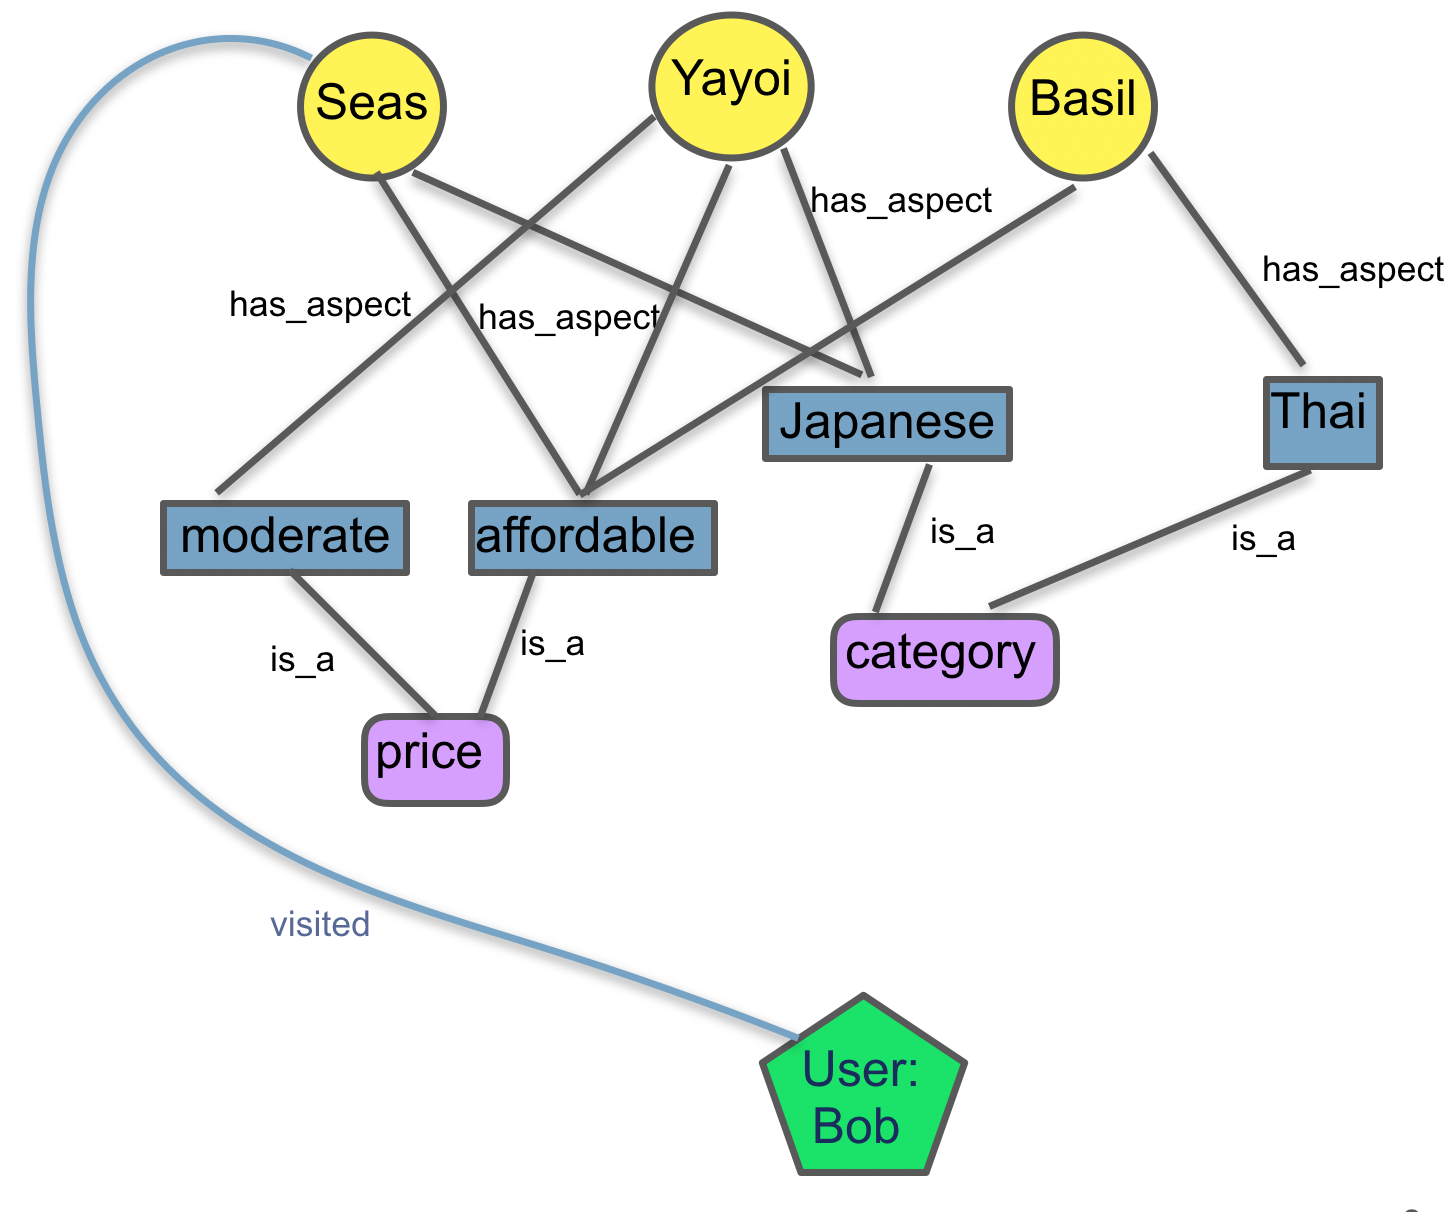
\includegraphics[width=5.5in]{fig/acl19_graph.png}
\caption{Construction of user memory graph}
\label{chap5:fig:graph}
\vspace{-15pt}
\end{figure}

\begin{figure}
\centering    
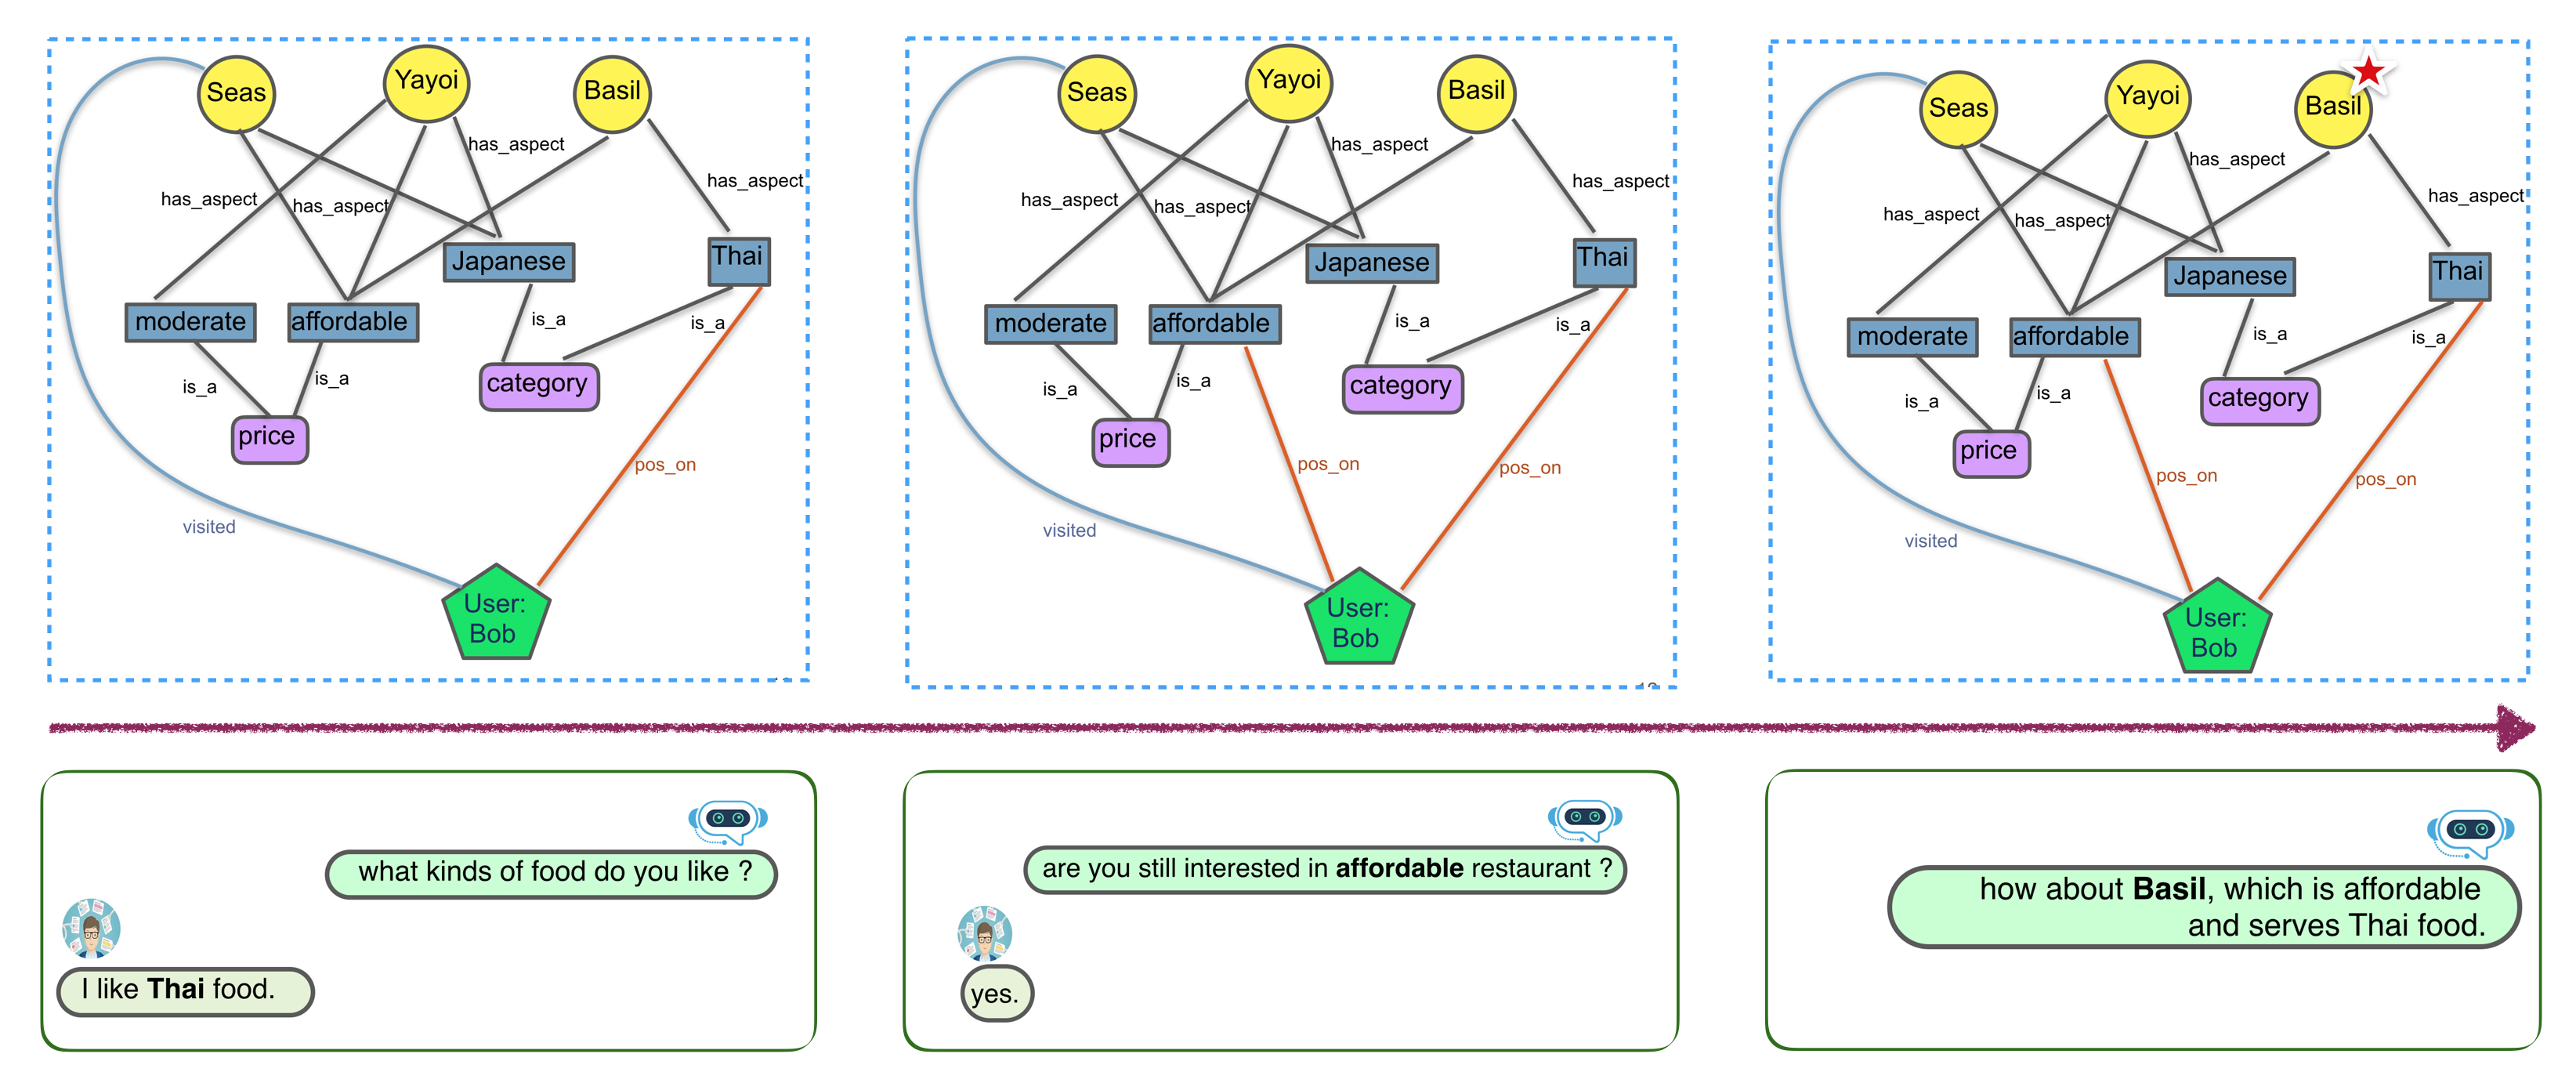
\includegraphics[width=6.0in]{fig/acl19_cum.png}
\caption{Dynamic updates of memory graph}
\label{chap5:fig:cum}
\vspace{-3mm}
\end{figure}

\section{Graph Reasoner}
\label{chap5:sec:umgr}

We propose a model called User Memory Graph Reasoner (UMGR) to reason the turn-level dialog policy over the user memory graph.\\ 
\textbf{Input}: the input of UMGR is the past dialog acts up to the current turn from the user $\boldsymbol{a}$, the updated user memory graph $\mathcal{G}'$, which contains all the knowledge about the items their associated values and slots, and visited items. We further accumulate all updates from the user (e.g., via the assumed results from NLU or state tracking) in the form of last 3 types of relations in Table 4 (Similar to visited items, we add a new memory entity for the current dialog and then associate all the new relations to that memory entity.).\\
\textbf{Output}: UMGR's output is the dialog policy $\pi=(\hat{y}^\mathcal{A}, \hat{y}^\mathcal{C}, \hat{y}^\mathcal{S}, \hat{y}^\mathcal{V})$ for the current turn, where $\mathcal{A}$, $\mathcal{C}$, $\mathcal{S}$, $\mathcal{V}$ indicate the space of dialog acts, candidate items, slots and values, respectively.
The predictions from $\hat{y}^\mathcal{C}, \hat{y}^\mathcal{S}$ and $\hat{y}^\mathcal{V}$ essentially provides a ranking over those entity sets.
For example, when $\hat{y}^\mathcal{A}=$ \textit{Recommendation}, the top-1 entity $\argmax_{e_i \in \mathcal{C}}(\hat{y}^\mathcal{C})$ will be provided to the user.
Similarly, $\hat{y}^\mathcal{A}=$ \textit{Open Question} is related to the top-1 slot $\argmax_{e_s \in \mathcal{S}}(\hat{y}^\mathcal{S})$ and $\hat{y}^\mathcal{A}=$ \textit{Yes/no Question} is related to the top-1 value $\argmax_{e_v \in \mathcal{V}}(\hat{y}^\mathcal{V})$.
In this way, all arguments of a dialog act can be mapped to certain entities in the user memory graph for a structured explanation instead of decoding from latent space.

To enable the reasoning over a user memory graph on-the-fly, we incorporate a Relational Graph Convolutional Networks (R-GCN) \cite{schlichtkrull2018modeling} inside UMGR.
R-GCN is a GCN \cite{kipf2016semi} with typed relations, where each relation is associated with their weights to enable reasoning over a heterogeneous graph.
UMGR first encodes past dialog acts $\boldsymbol{a}$ and entities $e \in \mathcal{E}$ into hidden dimensions.
%\vspace{-4mm}
\begin{equation}
\begin{split}
h_a = \text{LSTM}(W^\mathcal{A}(\boldsymbol{a})), \\
h_j^{(0)} = W^\mathcal{E}(e_j),
\end{split}
\end{equation}
where $W^\mathcal{A}$ and $W^\mathcal{E}$ are embedding layers and the past dialog acts are further encoded by an LSTM encoder.
We further allow on-the-fly reasoning over (new) items by sharing the embedding weights for different items (as a special entity \texttt{<ITEM>}) in $W^\mathcal{E}$. 
Then each entity in the user memory graph is encoded by multiple layers of R-GCN.
\begin{equation}
\begin{split}
h_j^{(l+1)}=\text{LeakyReLU} \Big(\sum_{r \in \mathcal{R}} \sum_{k \in \mathcal{N}_j^r} \frac{1}{\vert \mathcal{N}_j^r \vert} W_r^{(l)} h_j^{(l)}\Big),
\end{split}
\end{equation}
where $h_j^{(l)}$ ($j$ can be any type of entity) is the hidden state of entity $e_j$ in the $l$-th layer of R-GCN. $\mathcal{N}_j^r$ is entity $e_j$'s neighbor in relation type $r$ and $W_r^{(l)}$ is the weights associated with $r$ in the $l$-th layer to transform $h_j^{(l)}$.
The R-GCN layer updates the hidden states of each entity with the incoming messages in the form of their neighbors' hidden states type-by-type.
Then R-GCN sums over all types before passing through the activation.
The hidden states from the last layer of R-GCN is pasted into an aggregation layer.
\begin{equation}
\begin{split}
h^{\text{ag}} = \frac{1}{\vert \mathcal{C} \cup \mathcal{S} \cup \mathcal{V} \vert} \sum_{e_j \in \mathcal{C} \cup \mathcal{S} \cup \mathcal{V}} (W^\text{ag} h_j^{(l+1)} + b^{\text{ag}}),
\end{split}
\end{equation}
where $W^{\text{ag}}$ and $b^{\text{ag}}$ are weights for aggregation layer.
The purpose of having an aggregation layer is to leverage the information in the user memory graph for predicting the dialog acts, which is a classification problem. The loss for dialog acts is defined as
\begin{equation}
\begin{split}
\hat{y}^{\mathcal{A}} = \text{Softmax}(W^\mathcal{A} (h_a \oplus h^\text{ag}) +b^\mathcal{A} ), \\
\mathcal{L}^{\mathcal{A}} = \text{CrossEntropyLoss}(\hat{y}^\mathcal{A}, y^\mathcal{A}),
\end{split}
\end{equation}
where $\oplus$ is the concatenation operation and $y^\mathcal{A}$ is the annotated dialog act.
Further, all item, slot and value entities are trained by log loss for ranking. For example, the loss for candidate items $\mathcal{C}$ is defined as 
\begin{equation}
\begin{split}
\hat{y}_i = \text{Sigmoid}(W^\mathcal{I} h_i +b^{\mathcal{I}} ), \\
\mathcal{L}^\mathcal{C} = \text{LogLoss}(\hat{y}^\mathcal{C}, y^\mathcal{C}).
\end{split}
\end{equation}
Similarly, we obtain loses $\mathcal{L}_\mathcal{S}$, $\mathcal{L}_\mathcal{V}$ for slot entities $\mathcal{S}$ and value entities $\mathcal{V}$, respectively.
Finally, the total loss is the sum over all losses for dialog acts, items, slots and values: 
\begin{equation}
\begin{split}
\mathcal{L} = \mathcal{L}^\mathcal{A} + \alpha\mathcal{L}^\mathcal{C} + \beta\mathcal{L}^\mathcal{S} + \gamma \mathcal{L}^\mathcal{V},
\end{split}
\end{equation}
where $\alpha, \beta$ and $\gamma$ are hyper-parameters to align losses of different scales.
Note that during training and prediction, all invalid dialog acts (e.g., user dialog acts) and entities (e.g., not appear in a user memory graph) are masked out.
As we can see, unlike traditional recommender systems, UMGR does not learn (or ``overfit to'') any prior knowledge about users into the weights. Instead, it reasons the dialog policy on-the-fly in each turn based on the updated user memory graph.
We will detail the task of conversational recommendation and experiments in the next chapter.
